\chapter{First order equations} \label{fo:chapter}

%%%%%%%%%%%%%%%%%%%%%%%%%%%%%%%%%%%%%%%%%%%%%%%%%%%%%%%%%%%%%%%%%%%%%%%%%%%%%%

\section{Integrals as solutions}
\label{integralsols:section}

\sectionnotes{1 lecture (or less)\EPref{, \S1.2 in \cite{EP}}\BDref{,
covered in \S1.2 and \S2.1 in \cite{BD}}}

A first order ODE is an equation of the form
\begin{equation*}
\frac{dy}{dx} = f(x,y) ,
\end{equation*}
or just
\begin{equation*}
y' = f(x,y) .
\end{equation*}
In general, there is no simple formula or procedure one can follow to find
solutions.
In the next few lectures we will look at special cases where solutions are not
difficult to obtain.
In this section, let us assume that $f$ is a function of $x$ alone,
that is, the equation is
\begin{equation} \label{ias:inteq}
y' = f(x) .
\end{equation}
We could just integrate (antidifferentiate) both sides with respect to $x$.
\begin{equation*}
\int y'(x) \,dx = \int f(x) \,dx + C ,
\end{equation*}
that is
\begin{equation*}
y(x) = \int f(x) \,dx + C .
\end{equation*}
This $y(x)$ is actually the general solution.
So to solve \eqref{ias:inteq},
we find some antiderivative of $f(x)$
and then we add an arbitrary constant to get the general solution.

\begin{example}
Find the general solution of $y' = 3 x^2$.

Elementary calculus tells us
that the general solution must be $y = x^3 + C$.  Let us check by
differentiating:
$y' = 3x^2$.  We got \emph{precisely} our equation back.
\end{example}

Now is a good time to discuss a point about
calculus notation and terminology.  Calculus
textbooks muddy the waters by talking about the integral as primarily the
so-called indefinite integral.  The \myindex{indefinite integral}
is really the \emph{\myindex{antiderivative}} 
(in fact the whole one-parameter family
of antiderivatives).  There really exists only one integral and that
is the definite integral.
The only reason for the indefinite integral notation is that we can always
write an antiderivative as a (definite) integral.  That is, by the fundamental
theorem of calculus we can always write
$\int f(x) \,dx + C$ as
\begin{equation*}
\int_{x_0}^x f(t) \,dt + C .
\end{equation*}
Hence the terminology \emph{to \myindex{integrate}} when we may really mean
\emph{to \myindex{antidifferentiate}}.
Integration is just one way to compute the
antiderivative (and it is a way that always works, see the following
examples).  Integration is defined as the area under the graph, it
only happens to also compute antiderivatives.
For sake of consistency, we will keep using the
indefinite integral notation when we want an antiderivative,
and you should \emph{always} think of the definite integral
as a way to write it.

Normally, we also have an initial condition such as $y(x_0) = y_0$
for some two numbers $x_0$ and $y_0$ ($x_0$ is often 0, but not always).
We can then write the solution as a definite integral in a nice way.
Suppose our problem is $y' = f(x)$, $y(x_0) = y_0$.  Then the solution is
\begin{equation} \label{int:eqdef}
y(x) = \int_{x_0}^x f(t) \,dt + y_0 .
\end{equation}
Let us check!
We compute
$y' = f(x)$ via the fundamental theorem of calculus, and by Jupiter, $y$ is a
solution.  Is it the one satisfying the initial condition?  Well,
$y(x_0) = \int_{x_0}^{x_0} f(t)\,dt + y_0 = y_0$.  It is!

Do note that the definite integral and the indefinite integral
(antidifferentiation) are completely different beasts.  The definite integral
always evaluates to a number.  Therefore, \eqref{int:eqdef} is a formula we
can plug into the calculator or a computer, and it will be happy to calculate
specific values for us.  We will easily be able to plot the
solution and work with it just like with any other function.
It is not so crucial to always find a
closed form for the antiderivative.

\begin{example}
Solve
\begin{equation*}
y' = e^{-x^2}, \qquad y(0) = 1 .
\end{equation*}

By the preceding discussion, the solution must be
\begin{equation*}
y(x) = \int_0^x e^{-s^2} \,ds + 1 .
\end{equation*}
Here is a good way to make fun of your friends taking second semester
calculus.  Tell them to
find the closed form solution.  Ha ha ha (bad math joke).  It is
not possible (in closed form).
There is absolutely nothing wrong with writing the solution as a
definite integral.
This particular integral
is in fact very important
in statistics.
\end{example}

Using this method, we can also solve equations of the form
\begin{equation*}
y' = f(y) .
\end{equation*}
Let us write the equation in \myindex{Leibniz notation}.
\begin{equation*}
\frac{dy}{dx} = f(y) .
\end{equation*}
Now we use the inverse function theorem from calculus
to switch the roles of $x$ and $y$
to obtain
\begin{equation*}
\frac{dx}{dy} = \frac{1}{f(y)} .
\end{equation*}
What
we are doing seems like algebra with $dx$ and $dy$.
It is tempting to just do algebra with $dx$
and $dy$ as if they were numbers.  And in this case it does work.  Be
careful,
however, as this sort of hand-waving calculation can lead to trouble,
especially when
more than one independent variable is involved.
At this point, we can simply integrate,
\begin{equation*}
x(y) = \int \frac{1}{f(y)} \,dy + C .
\end{equation*}
Finally, we try to solve for $y$.

\begin{example}
Previously, we guessed $y' = ky$ (for some $k > 0$) has the solution
$y=Ce^{kx}$.  We could have found the solution by integrating.
First we note that $y=0$ is a solution.
Henceforth, we assume $y\not= 0$.  We write
\begin{equation*}
\frac{dx}{dy} = \frac{1}{ky} .
\end{equation*}
We integrate to obtain
\begin{equation*}
x(y) = x = \frac{1}{k} \ln \, \lvert y \rvert + D,
\end{equation*}
where $D$ is an arbitrary constant.
Now we solve for $y$ (actually for $\lvert y \rvert$).
\begin{equation*}
\lvert y \rvert =
e^{kx-kD} = 
e^{-kD} e^{k x} .
\end{equation*}
If we replace $e^{-kD}$ with an arbitrary constant $C$, we can
get rid of the absolute value bars (which we can do as $D$ was arbitrary).  In
this way, we
also incorporate the solution $y=0$.  We get the same general solution as
we guessed before, $y = Ce^{kx}$.
\end{example}

\begin{example}
Find the general solution of
$y' = y^2$.

First we note that $y=0$ is a solution.  We can now assume that $y \not= 0$.
Write
\begin{equation*}
\frac{dx}{dy} = \frac{1}{y^2} .
\end{equation*}
We integrate to get
\begin{equation*}
x = \frac{-1}{y} + C .
\end{equation*}
We solve for $y = \frac{1}{C-x}$.
So the general solution is
\begin{equation*}
y = \frac{1}{C-x} \qquad \text{or} \qquad y = 0.
\end{equation*}
Note the singularities of the solution.  If, for example, $C=1$, then the
solution \myquote{blows up} as we approach $x=1$.  See
\figurevref{1over1mx:fig}.  Generally,
it is hard to tell
from just looking at the equation itself how the solution is going to behave.
The equation $y' = y^2$ is very nice and defined everywhere, but
the solution is only defined on some interval $(-\infty, C)$ or
$(C, \infty)$.  Usually when this happens we only consider one of these
the solution.  For example if we impose a condition $y(0) = 1$, then
the solution is $y=\frac{1}{1-x}$, and we would consider this solution only
for $x$ on the interval $(-\infty,1)$.  In the figure, it is the left side
of the graph.
\begin{myfig}
\capstart
\diffyincludegraphics{width=3in}{width=4.5in}{1over1mx}
\caption{Plot of $y=\frac{1}{1-x}$.\label{1over1mx:fig}}
\end{myfig}
\end{example}

Classical problems leading to differential equations solvable by integration
are problems 
dealing with \myindex{velocity},
\myindex{acceleration} and \myindex{distance}.  You have surely seen these
problems before in your calculus class.

\begin{example}
Suppose a car drives at a speed $e^{t/2}$ meters per second,
where $t$ is time in seconds.
How far did the car get in 2 seconds (starting at $t=0$)?  How far in 10 seconds?

Let $x$ denote the distance the car traveled.
The equation is
\begin{equation*}
x' = e^{t/2} .
\end{equation*}
We just integrate this equation to get that
\begin{equation*}
x(t) = 2 e^{t/2} + C . 
\end{equation*}
We still need to figure out $C$.  We know that when $t=0$, then
$x=0$.  That is, $x(0) = 0$.  So
\begin{equation*}
0 = x(0) = 2e^{0/2} + C = 2 + C .
\end{equation*}
Thus $C = -2$ and 
\begin{equation*}
x(t) = 2 e^{t/2} - 2 .
\end{equation*}
Now we just plug in to get where the car is at 2 and at 10 seconds.
We obtain
\begin{equation*}
x(2) = 2e^{2/2} - 2 \approx 3.44 \text{ meters} ,
\qquad
x(10) = 2e^{10/2} - 2 \approx 294 \text{ meters} .
\end{equation*}
\end{example}

\begin{example}
Suppose that the car accelerates at a rate of $\unitfrac[t^2]{m}{s^2}$.
At time $t=0$ the car is at the 1 meter mark and is traveling at
\unitfrac[10]{m}{s}.  Where is the car at time $t=10$?

Well this is actually a second order problem.  If $x$ is the distance
traveled, then $x'$ is the velocity, and $x''$ is the acceleration.
The equation with initial conditions is
\begin{equation*}
x'' = t^2 , \qquad x(0) = 1 , \qquad x'(0) = 10 .
\end{equation*}
What if we say $x' = v$.  Then we have the problem
\begin{equation*}
v' = t^2, \qquad v(0) = 10 .
\end{equation*}
Once we solve for $v$, we can integrate and find $x$.
\end{example}

\begin{exercise}
Solve for $v$, and then solve for $x$.  Find $x(10)$ to answer the
question.
\end{exercise}

\subsection{Exercises}

\begin{exercise}
Solve $\frac{dy}{dx} = x^2+x$ for $y(1)=3$.
\end{exercise}

\begin{exercise}
Solve $\frac{dy}{dx} = \sin (5x)$ for $y(0)=2$.
\end{exercise}

\begin{exercise}
Solve $\frac{dy}{dx} = \frac{1}{x^2-1}$ for $y(0)=0$.
\end{exercise}

\begin{exercise}
Solve $y' = y^3$ for $y(0)=1$.
\end{exercise}

\begin{exercise}[little harder]
Solve $y' = (y-1)(y+1)$ for $y(0)=3$.
\end{exercise}

\begin{exercise}
Solve $\frac{dy}{dx} = \frac{1}{y+1}$ for $y(0)=0$.
\end{exercise}

\begin{exercise}[harder]
Solve $y'' = \sin x$ for $y(0)=0$, $y'(0) = 2$.
\end{exercise}

\begin{exercise}
A spaceship is traveling at the speed \unitfrac[$2t^2+1$]{km}{s} ($t$ is
time in seconds).  It is pointing directly away from earth and at time $t=0$
it is 1000 kilometers from earth.  How far from earth is it at one minute from
time $t=0$?
\end{exercise}

\begin{exercise}
Solve $\frac{dx}{dt} = \sin(t^2)+t$, $x(0)=20$.  It is OK to leave your
answer as a definite integral.
\end{exercise}

\begin{exercise}
A dropped ball accelerates downwards at a constant rate $9.8$ meters per second
squared.  Set up the differential equation for the height above ground $h$ in meters.
Then supposing $h(0) = 100$ meters, how long does it take for the ball to hit
the ground.
\end{exercise}

\begin{exercise}
Find the general solution of
$y' = e^x$,  and then $y' = e^y$.
\end{exercise}


\setcounter{exercise}{100}

\begin{exercise}
Solve $\frac{dy}{dx} = e^x + x$ and $y(0) = 10$.
\end{exercise}
\exsol{%
$y = e^x + \frac{x^2}{2} + 9$
}

\begin{exercise}
Solve $x' = \frac{1}{x^2}$, $x(1)=1$.
\end{exercise}
\exsol{%
$x = {(3t-2)}^{1/3}$
}

\begin{exercise}
Solve $x' = \frac{1}{\cos(x)}$, $x(0)=\frac{\pi}{4}$.
\end{exercise}
\exsol{%
$x = \sin^{-1} \bigl(t+\nicefrac{1}{\sqrt{2}}\bigr)$
}

\begin{exercise}
Sid is in a car traveling at speed $10t+70$ miles per hour away from Las Vegas,
where $t$ is in hours.  At $t=0$, Sid is 10 miles away from Vegas.  How
far from Vegas is Sid 2 hours later?
\end{exercise}
\exsol{%
170
}

\begin{exercise}
Solve $y' = y^n$, $y(0) = 1$, where $n$ is a positive integer.
Hint: You have to consider different cases.
\end{exercise}
\exsol{%
If $n \not= 1$, then
$y={\bigl((1-n)x+1\bigr)}^{1/(1-n)}$.
If $n=1$, then $y = e^x$.
}

\begin{exercise}
The rate of change of the volume of a snowball that is melting is 
proportional to the surface area of the snowball.  Suppose the
snowball is perfectly spherical.  The volume (in centimeters cubed)
of a ball of radius $r$ centimeters is
$(\nicefrac{4}{3}) \pi r^3$.  The surface area is
$4 \pi r^2$.  Set up the differential equation for how the radius $r$ is changing.
Then, suppose that at time $t=0$ minutes, the radius is 10 centimeters.
After 5 minutes, the radius is 8 centimeters.  At what time $t$ will the 
snowball be completely melted?
\end{exercise}
\exsol{%
The equation is $r' = -C$ for some constant $C$.
The snowball will be completely melted in 25 minutes from time $t=0$.
}

\begin{exercise}
Find the general solution to $y''''= 0$.  How many distinct constants do you need?
\end{exercise}
\exsol{%
$y = Ax^3 + Bx^2 + Cx + D$, so 4 constants.
}

%%%%%%%%%%%%%%%%%%%%%%%%%%%%%%%%%%%%%%%%%%%%%%%%%%%%%%%%%%%%%%%%%%%%%%%%%%%%%%

\sectionnewpage
\section{Slope fields}
\label{slopefields:section}

\sectionnotes{1 lecture\EPref{, \S1.3 in \cite{EP}}\BDref{,
\S1.1 in \cite{BD}}}

%At this point it may be good to first try the
%Lab I\index{IODE software!Lab I} and/or Project I\index{IODE software!Project I} from the
%IODE website: \url{http://www.math.uiuc.edu/iode/}.
%
%\medskip

As we said, the general first order equation we are studying looks like
\begin{equation*}
y' = f(x,y).
\end{equation*}
A lot of the time, we cannot simply solve these kinds of equations explicitly.
It would be nice if we could at least figure out the shape and behavior of
the solutions, or find approximate solutions.

\subsection{Slope fields}

%As you have seen in IODE Lab I (if you did it),
The equation $y' = f(x,y)$
gives you a slope at each point 
in the
$(x,y)$-plane.  And this is the slope a solution $y(x)$ would have 
at $x$ if its value was $y$.  In other words, $f(x,y)$ is the slope
of a solution whose graph runs through the
point $(x,y)$.  At a point $(x,y)$, we plot a short line
with the slope $f(x,y)$.
For example, if $f(x,y) = xy$, then at point $(2,1.5)$ we draw a
short line of slope $xy = 2 \times 1.5 = 3$.  So, if $y(x)$ is a solution
and $y(2) = 1.5$, then the equation mandates that $y'(2) = 3$.
See \figurevref{1.3:fig0}.

\begin{myfig}
\capstart
\diffyincludegraphics{width=3in}{width=4.5in}{1-3-xysl-one}
\caption{The slope $y'=xy$ at $(2,1.5)$.\label{1.3:fig0}}
\end{myfig}

To get an idea of how solutions behave, we draw such lines at lots
of points in the plane, not just the point $(2,1.5)$.  We would
ideally want to see the slope at every point, but that is
just not possible.  Usually we pick a
grid of points fine enough so that it shows the behavior, but not too
fine so that we can still recognize the individual lines.
We call this picture the \emph{\myindex{slope field}} of the equation.
See \figurevref{1.3:fig1} for the slope field of the equation $y' = xy$.
Usually in practice, one does not do this by hand, but has a computer do the
drawing.

Suppose we are given a specific initial condition $y(x_0) = y_0$.
A solution, that is, the graph of the solution, would be a curve
that follows the slopes we drew.
For a few sample
solutions, see \figurevref{1.3:fig2}.  It is easy to roughly sketch
(or at least imagine)
possible solutions in the slope field, just from looking at the slope field
itself.  You simply sketch a line that roughly fits the little line segments
and goes through your initial condition.

\begin{myfig}
\parbox[t]{3.0in}{
 \capstart
 \diffyincludegraphics{width=3.0in}{width=4.5in}{1-3-xysl}
 \caption{Slope field of $y' = xy$.\label{1.3:fig1}}
}
\quad
\parbox[t]{3.0in}{
 \capstart
 \diffyincludegraphics{width=3.0in}{width=4.5in}{1-3-xysl-sol}
 \caption{Slope field of $y' = xy$ with a graph of solutions satisfying
 $y(0) = 0.2$, $y(0) = 0$, and $y(0) = -0.2$.\label{1.3:fig2}}
}
\end{myfig}

By looking at the slope field we get a lot of information
about the behavior of solutions without having to solve
the equation.  For
example, in \figurevref{1.3:fig2} we see what the solutions do when the initial conditions
are $y(0) > 0$, $y(0) = 0$ and $y(0) < 0$.
A small change in the
initial condition causes quite different behavior.
We see this behavior just
from the slope field and imagining what solutions ought to do.

We see a different behavior for the equation
$y' = -y$.  The slope field and a few solutions is in
see \figurevref{1.3:fig3}.
If we think of moving from left to right (perhaps $x$ is time
and time is usually increasing), then
we see that no matter what $y(0)$ is, all solutions tend to zero as $x$
tends to infinity.
Again that behavior is clear from simply
looking at the slope field itself.

\begin{myfig}
\capstart
\diffyincludegraphics{width=3in}{width=4.5in}{1-3-mysl-sol}
\caption{Slope field of $y' = -y$ with a graph of a few solutions.\label{1.3:fig3}}
\end{myfig}

\subsection{Existence and uniqueness}

We wish to ask two fundamental questions about the problem
\begin{equation*}
y' = f(x,y), \qquad y(x_0) = y_0.
\end{equation*}
\begin{enumerate}[(i)]
\item Does a solution \emph{exist}?
\item Is the solution \emph{unique} (if it exists)?
\end{enumerate}

What do you think is the answer?
The answer seems to be yes to both does it not?  Well, pretty much.  But there
are cases when the answer to either question can be no.

Since generally the equations we encounter in applications
come from real life situations, it seems
logical that a solution always exists.
It also has to be unique if we believe our
universe is deterministic.  If the solution does not exist, or if it is
not unique, we have
probably not devised the correct model.  Hence, it is good to know
when things go wrong and why.

\begin{example}
Attempt to solve:
\begin{equation*}
y' = \frac{1}{x}, \qquad y(0) = 0 .
\end{equation*}

Integrate to find the general solution $y = \ln \, \lvert x \rvert + C$.  The
solution does not exist at $x=0$.  See \figurevref{1.3:xinvfig}.
The equation may have been written as the seemingly harmless $x y' = 1$.

\begin{myfig}
\parbox[t]{3in}{
 \capstart
 \diffyincludegraphics{width=3in}{width=4.5in}{1-3-xinv-sol}
 \caption{Slope field of $y' = \nicefrac{1}{x}$.\label{1.3:xinvfig}}
}
\quad
\parbox[t]{3in}{
 \capstart
 \diffyincludegraphics{width=3in}{width=4.5in}{1-3-sqrt-sol}
 \caption{Slope field of $y' = 2 \sqrt{\lvert y \rvert}$ with two
 solutions satisfying $y(0) = 0$.\label{1.3:sqrtfig}}
}
\end{myfig}
\end{example}

\begin{example}
Solve:
\begin{equation*}
y' = 2 \sqrt{\lvert y \rvert}, \qquad y(0) = 0 .
\end{equation*}

See \figurevref{1.3:sqrtfig}.
Note that $y=0$ is a solution.  But another solution is the function
\begin{equation*}
y(x) =
\begin{cases}
x^2 & \text{if } \; x \geq 0,\\
-x^2 & \text{if } \; x < 0.
\end{cases}
\end{equation*}
\end{example}

It is hard to tell by staring at the slope field that the
solution is not
unique.
Is there any hope?
Of course there is.  We have the following theorem,
known as Picard's theorem%
\footnote{Named after the French mathematician
\href{https://en.wikipedia.org/wiki/Charles_\%C3\%89mile_Picard}{Charles \'Emile Picard}
(1856--1941)}. 

\begin{theorem}[Picard's theorem on existence and uniqueness]%
\label{slope:picardthm}%
\index{existence and uniqueness}\index{Picard's theorem}
If $f(x,y)$ is continuous (as a function of two
variables) and $\frac{\partial f}{\partial y}$ exists and is
continuous near some $(x_0,y_0)$, then a solution to
\begin{equation*}
y' = f(x,y), \qquad y(x_0) = y_0,
\end{equation*}
exists (at least for $x$ in some small interval) and is unique.
\end{theorem}

Note that the problems $y' = \nicefrac{1}{x}$, $y(0) = 0$ and 
$y' = 2 \sqrt{\lvert y \rvert}$, $y(0) = 0$ do not satisfy the hypothesis of the
theorem.
Even if we can use the theorem,
we ought to be careful about this existence business.  It is quite
possible that the solution only exists for a short while.

\begin{example}
For some constant $A$, solve:
\begin{equation*}
y' = y^2, \qquad y(0) = A .
\end{equation*}

We know how to solve this equation.  First assume that $A \not= 0$,
so $y$ is not equal to zero at least for some $x$ near 0.  So
$x' = \nicefrac{1}{y^2}$, so
$x = \nicefrac{-1}{y} + C$, so $y = \frac{1}{C-x}$.  If $y(0) = A$, then
$C = \nicefrac{1}{A}$ so
\begin{equation*}
y = \frac{1}{\nicefrac{1}{A} - x} .
\end{equation*}
If $A=0$, then $y=0$ is a solution.

For example, when $A=1$
the solution \myquote{blows up} at $x=1$.  Hence, the solution does not exist
for all $x$ even if the equation is nice everywhere.  The equation
$y' = y^2$ certainly
looks nice.
\end{example}

For most of this
course we will be interested in equations where existence and
uniqueness holds, and in fact holds \myquote{globally} unlike for the equation
$y'=y^2$.
%But it is necessary to understand the examples where things fail for the
%aforementioned reasons.

\subsection{Exercises}

\begin{exercise}
Sketch slope field for $y'=e^{x-y}$.  How do the solutions behave as $x$
grows?  Can you guess a particular solution by looking at the slope
field?
\end{exercise}

\begin{exercise}
Sketch slope field for $y'=x^2$.
\end{exercise}

\begin{exercise}
Sketch slope field for $y'=y^2$.
\end{exercise}

\begin{exercise}
Is it possible to solve the equation $y' = \frac{xy}{\cos x}$ for $y(0) = 1$?
Justify.
\end{exercise}

\begin{exercise}
Is it possible to solve the equation $y' = y\sqrt{\lvert x\rvert}$ for
$y(0) = 0$?  Is the solution unique?
Justify.
\end{exercise}

\begin{samepage}
\begin{exercise}
Match equations $y'=1-x$, $y'=x-2y$, $y' = x(1-y)$ to slope fields.
Justify.
\begin{tasks}(3)
\task
\parbox[c]{1.75in}{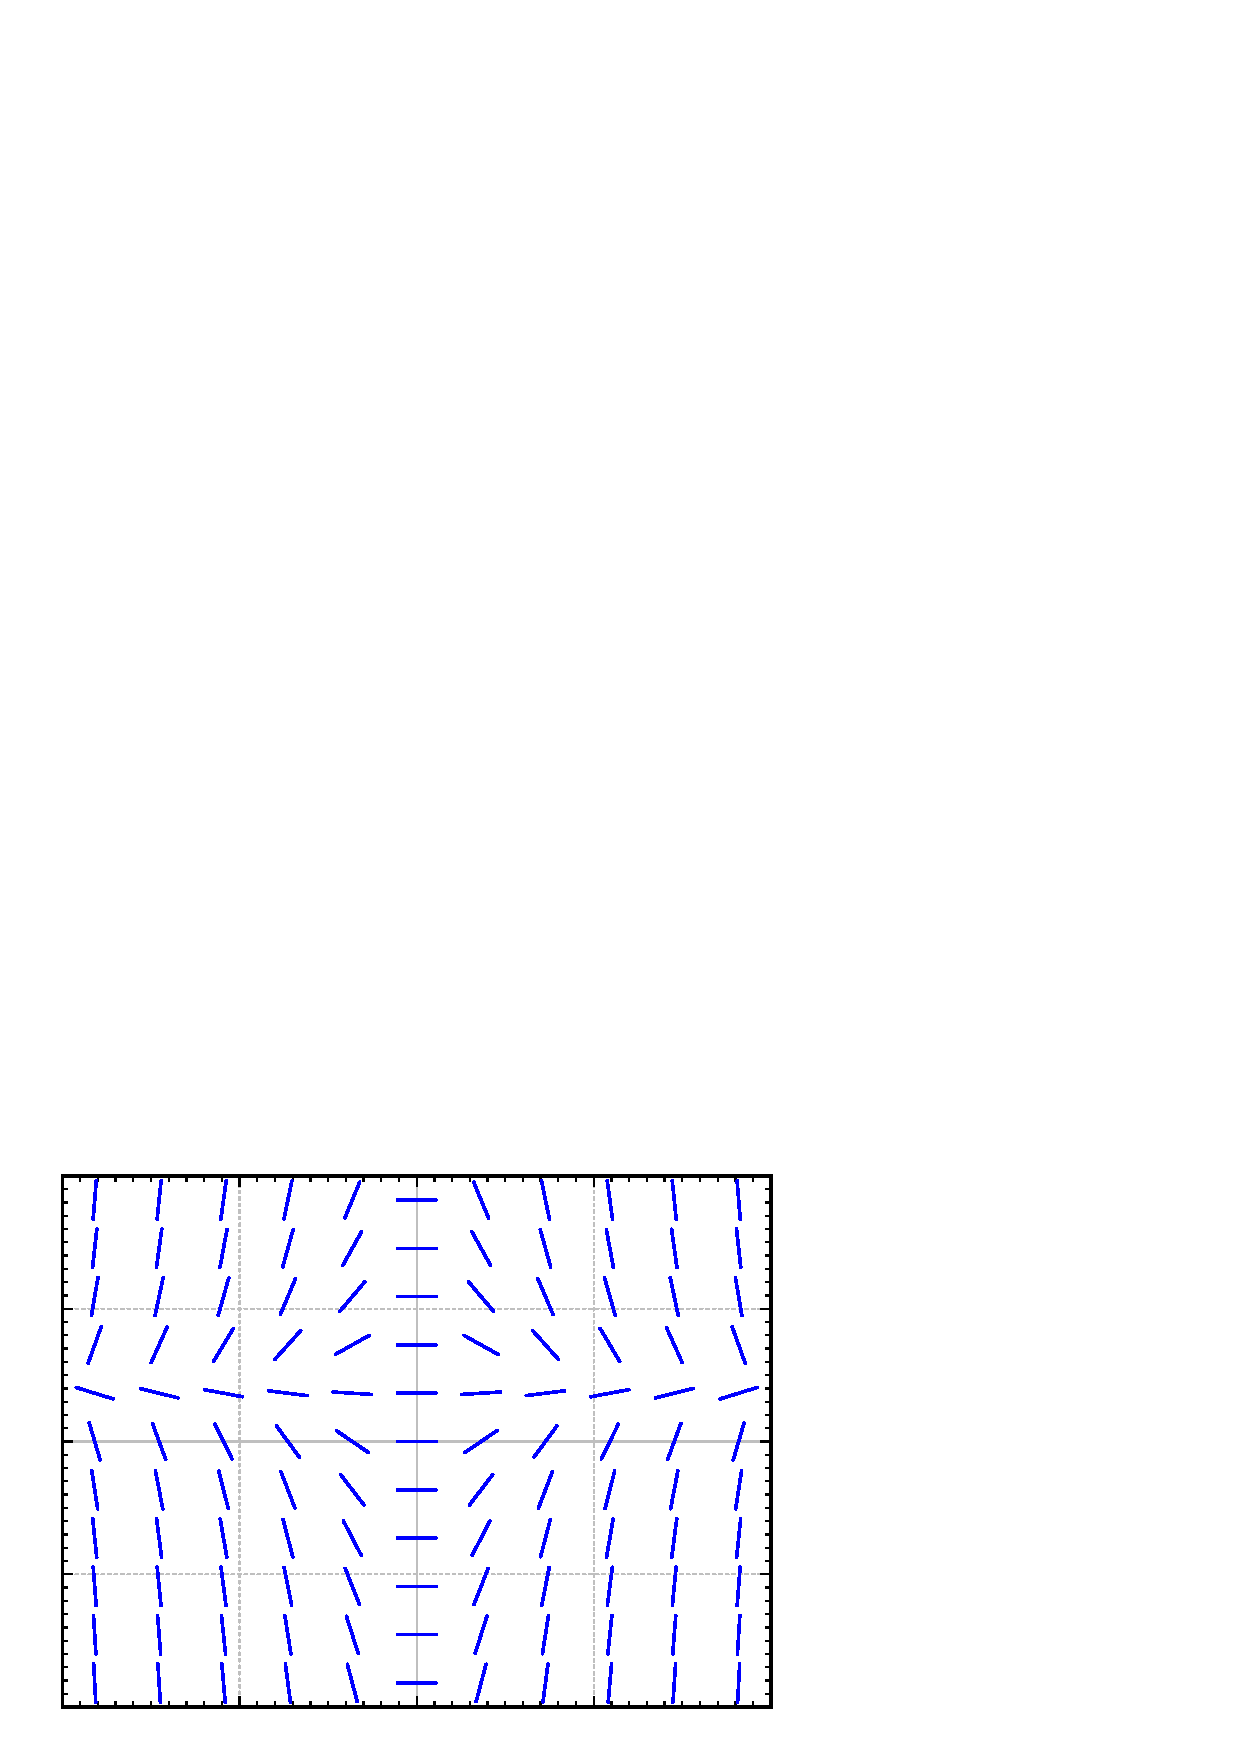
\includegraphics[width=1.75in]{figures/yprimex1minusyslope}}
\task
\parbox[c]{1.75in}{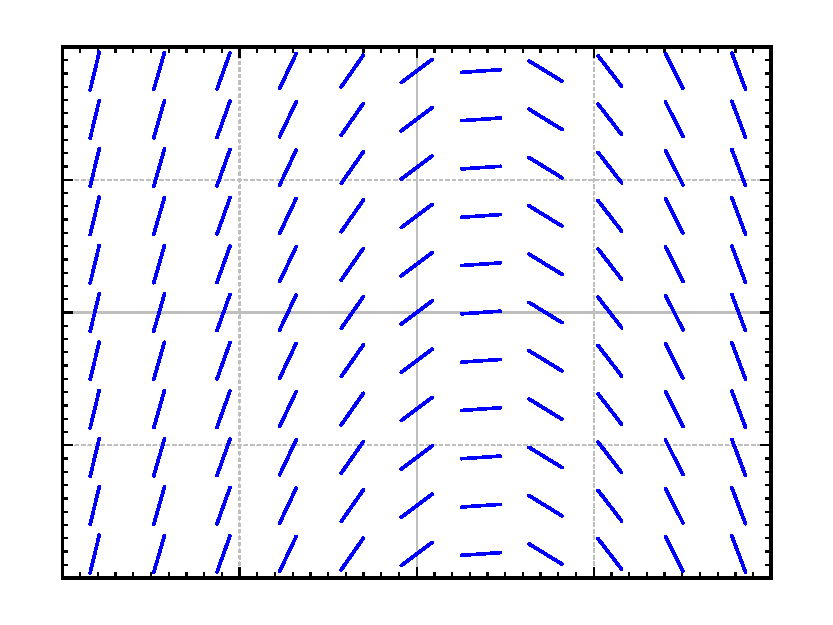
\includegraphics[width=1.75in]{figures/yprime1minusxslope}}
\task
\parbox[c]{1.75in}{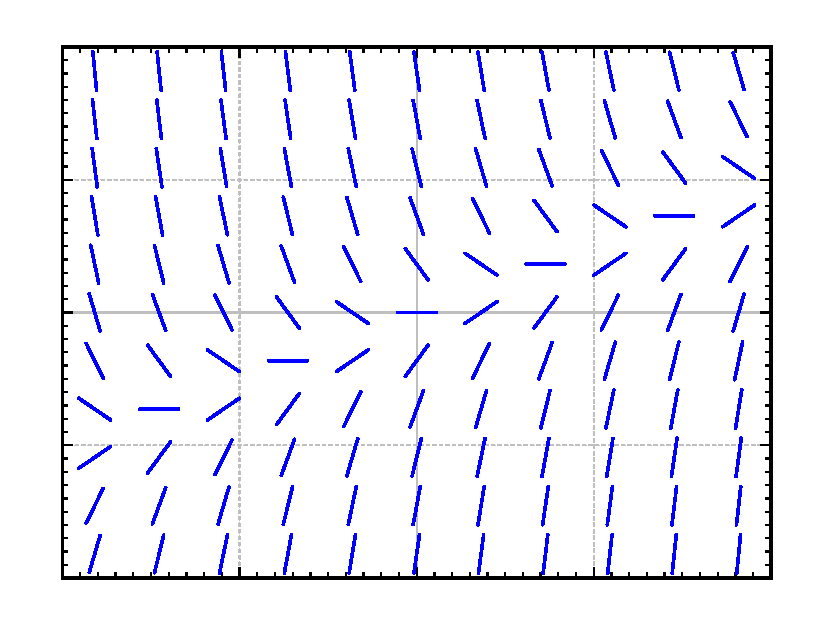
\includegraphics[width=1.75in]{figures/yprimexminus2yslope}}
\end{tasks}
\end{exercise}
\end{samepage}

\begin{exercise}[challenging]
Take $y' = f(x,y)$, $y(0) = 0$, where $f(x,y) > 1$
for all $x$ and $y$.  If
the solution exists for all $x$, can you say
what happens to $y(x)$ as $x$ goes to positive infinity?  Explain.
\end{exercise}

\begin{exercise}[challenging]
Take $(y-x)y' = 0$, $y(0) = 0$.
\begin{tasks}
\task Find two distinct solutions.
\task Explain why this does not violate Picard's theorem.  
\end{tasks}
\end{exercise}

\begin{exercise}
Suppose $y' = f(x,y)$.  What will the slope field look like, explain and
sketch an example, if you know the following about $f(x,y)$:
\begin{tasks}(2)
\task $f$ does
not depend on $y$.
\task $f$ does not depend on $x$.
\task $f(t,t) = 0$ for any
number $t$.
\task $f(x,0) = 0$ and $f(x,1) = 1$ for all $x$.
\end{tasks}
\end{exercise}

\begin{exercise}
Find a solution to $y' = \lvert y \rvert$, $y(0) = 0$.  Does Picard's theorem apply?
\end{exercise}

\begin{exercise}
Take an equation $y' = (y-2x) g(x,y) + 2$ for some function $g(x,y)$.
Can you solve the problem for the
initial condition $y(0) = 0$,
and if so what is the solution?
\end{exercise}

\begin{exercise}[challenging]
\pagebreak[2]
Suppose $y' = f(x,y)$ is such that $f(x,1) = 0$ for every $x$,
$f$ is continuous and $\frac{\partial f}{\partial y}$ exists and
is continuous for every $x$ and $y$.
\begin{tasks}
\task
Guess a solution given the initial condition
$y(0) = 1$.
\task
Can graphs of two solutions of the equation for different initial conditions
ever intersect?
\task
Given $y(0) = 0$, what can you say about the solution.  In particular,
can $y(x) > 1$ for any $x$?  Can $y(x) = 1$ for any $x$?  Why or why not?
\end{tasks}
\end{exercise}

\setcounter{exercise}{100}

\begin{exercise}
Sketch the slope field of $y'=y^3$.  Can you visually find the solution
that satisfies $y(0)=0$?
\end{exercise}
\exsol{%
%mbxSTARTIGNORE
\vtop{\vskip-1ex \hbox{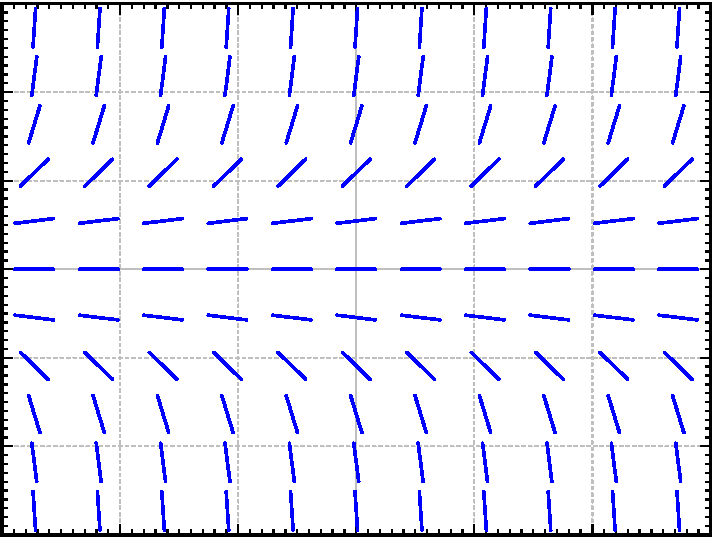
\includegraphics[width=2in]{figures/yprimey3slope}}}
\quad
%mbxENDIGNORE
%mbxlatex \\
%mbxlatex 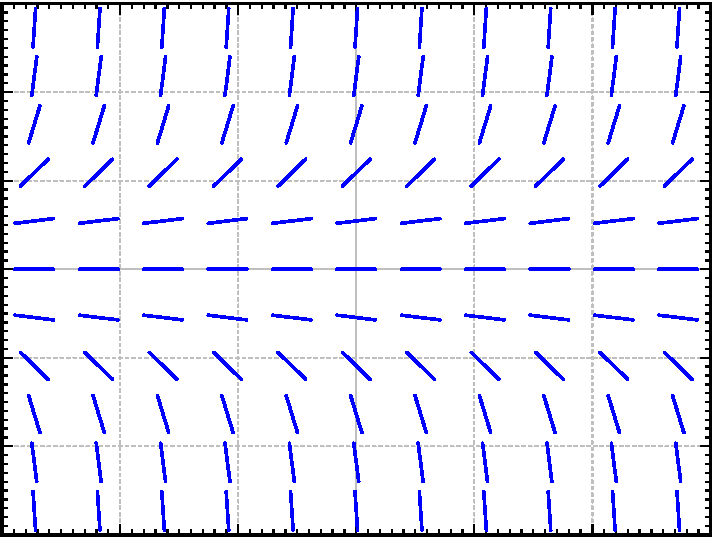
\includegraphics[width=2in]{figures/yprimey3slope}
%mbxlatex \\
$y=0$ is a solution such that $y(0)=0$.
}

\begin{exercise}
Is it possible to solve $y' = xy$ for $y(0) = 0$?  Is the solution unique?
\end{exercise}
\exsol{%
Yes a solution exists.  The equation is $y' = f(x,y)$ where $f(x,y) = xy$.  The function
$f(x,y)$ is continuous and 
$\frac{\partial f}{\partial y} = x$, which is also continuous near $(0,0)$.
So a solution exists and is unique.  (In fact, $y=0$ is the solution.)
}

\begin{exercise}
Is it possible to solve $y' = \frac{x}{x^2-1}$ for $y(1) = 0$?
\end{exercise}
\exsol{%
No, the equation is not defined at $(x,y) = (1,0)$.
}

\begin{samepage}
\begin{exercise}
Match equations $y'=\sin x$, $y'=\cos y$, $y' = y\cos(x)$ to slope fields.
Justify.
\begin{tasks}(3)
\task
\parbox[c]{1.75in}{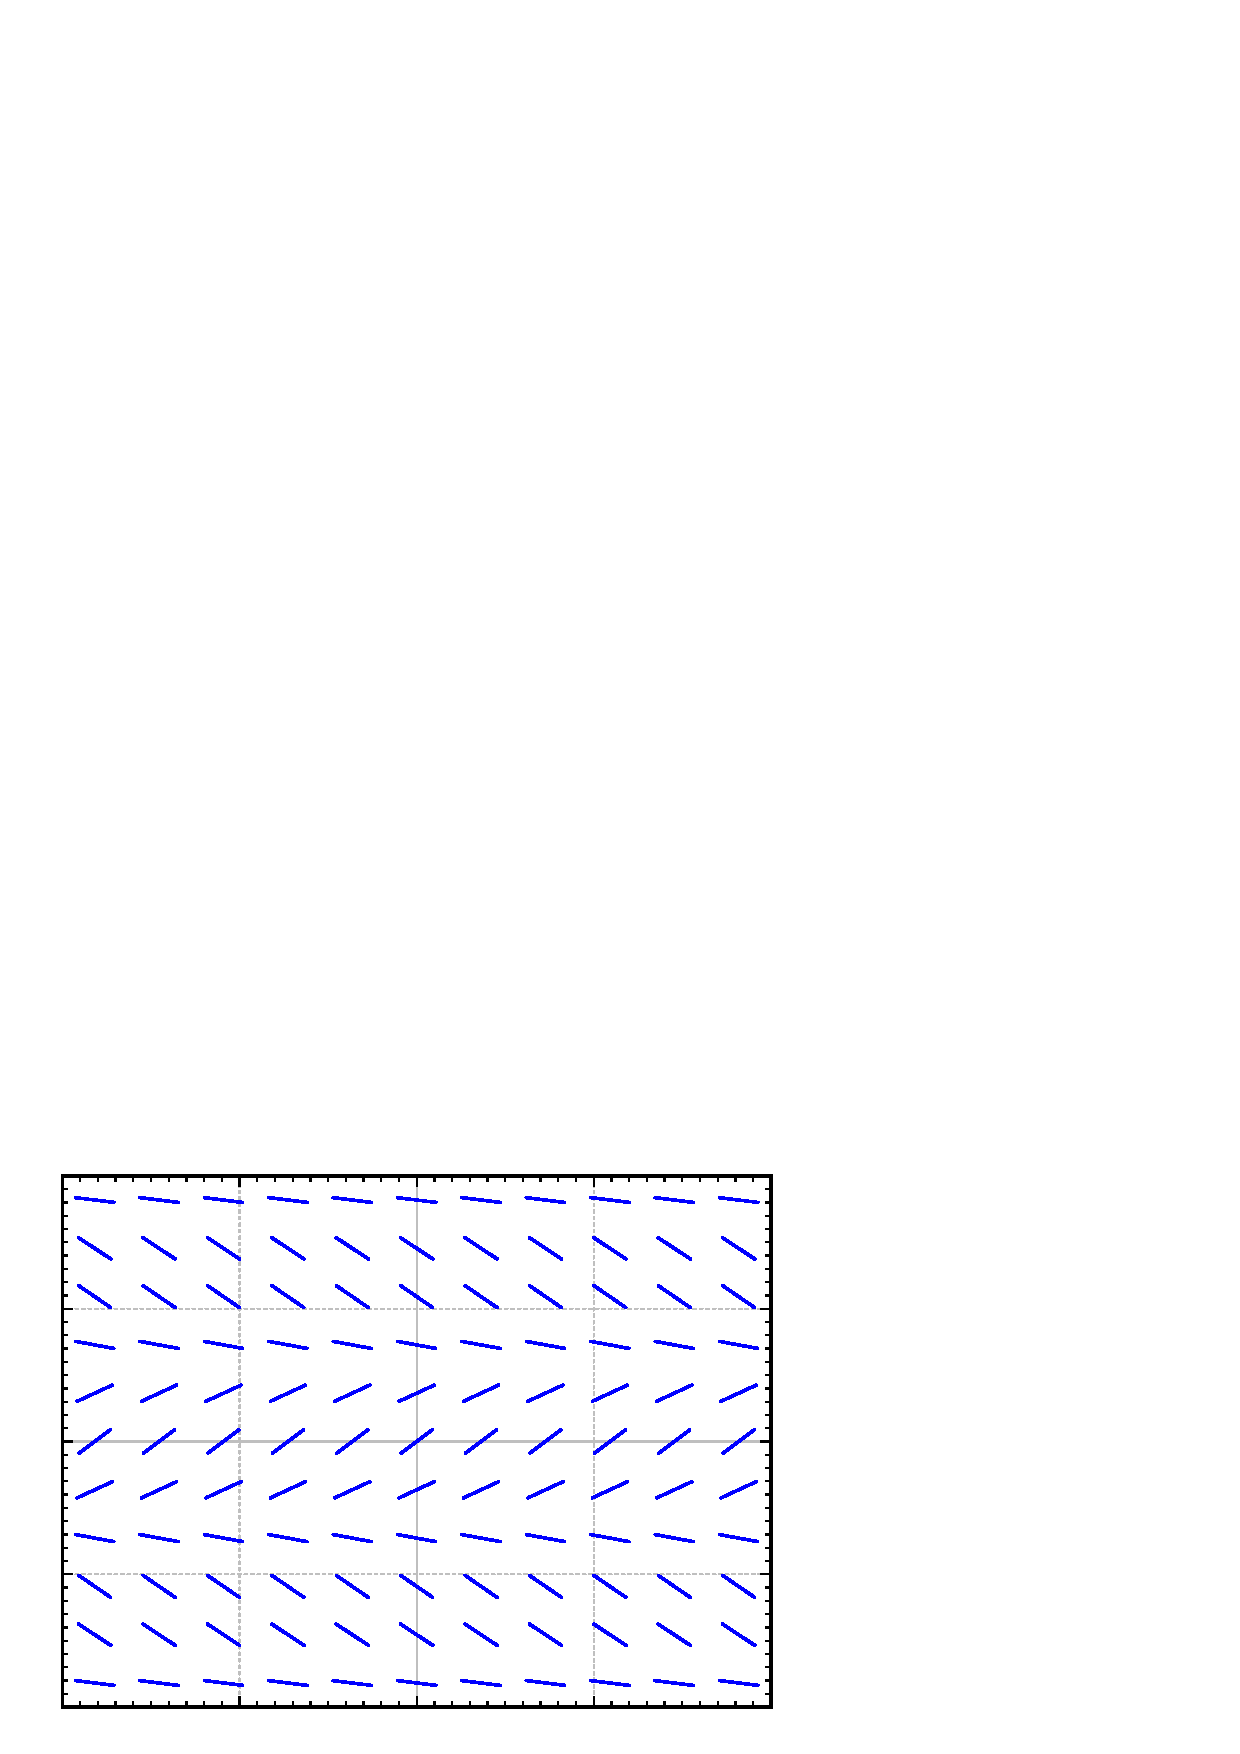
\includegraphics[width=1.75in]{figures/yprimecosyslope}}
\task
\parbox[c]{1.75in}{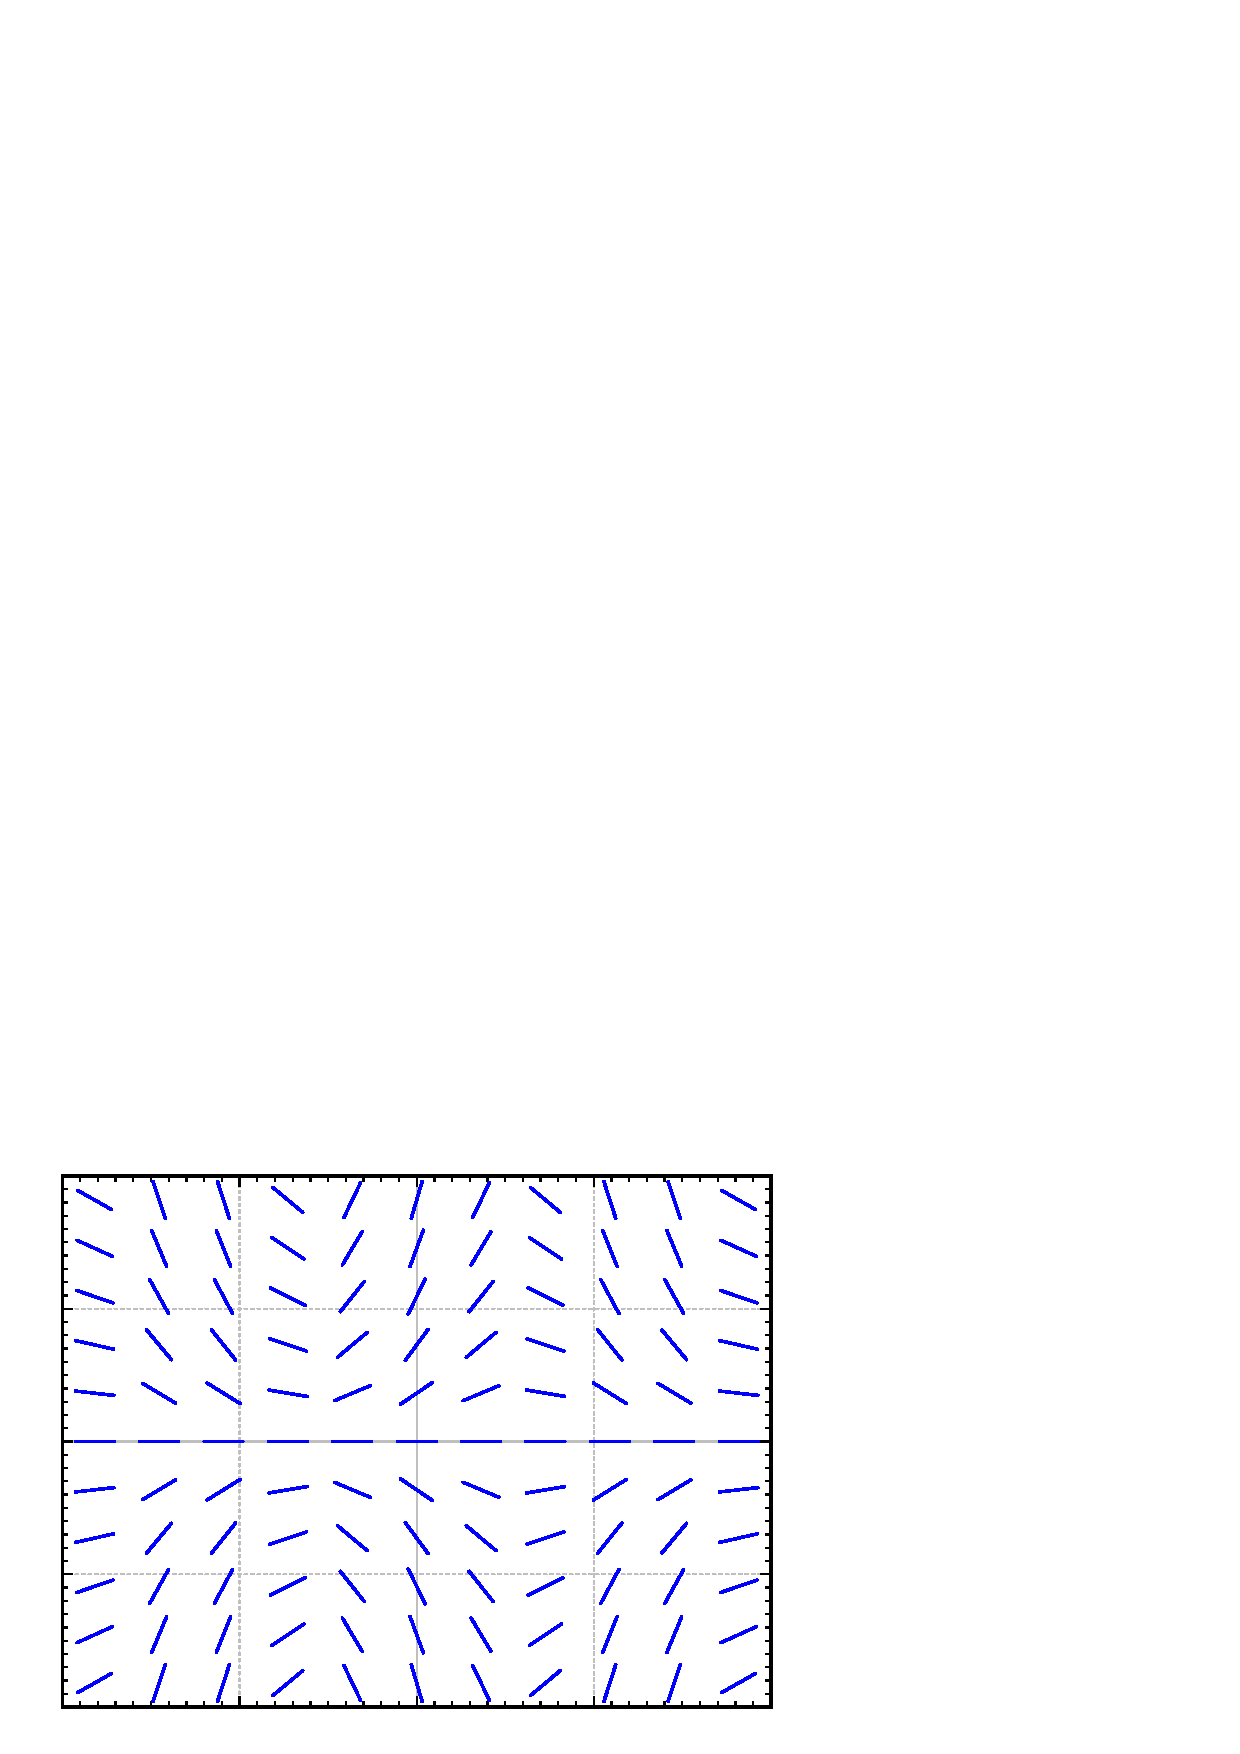
\includegraphics[width=1.75in]{figures/yprimecosxyslope}}
\task
\parbox[c]{1.75in}{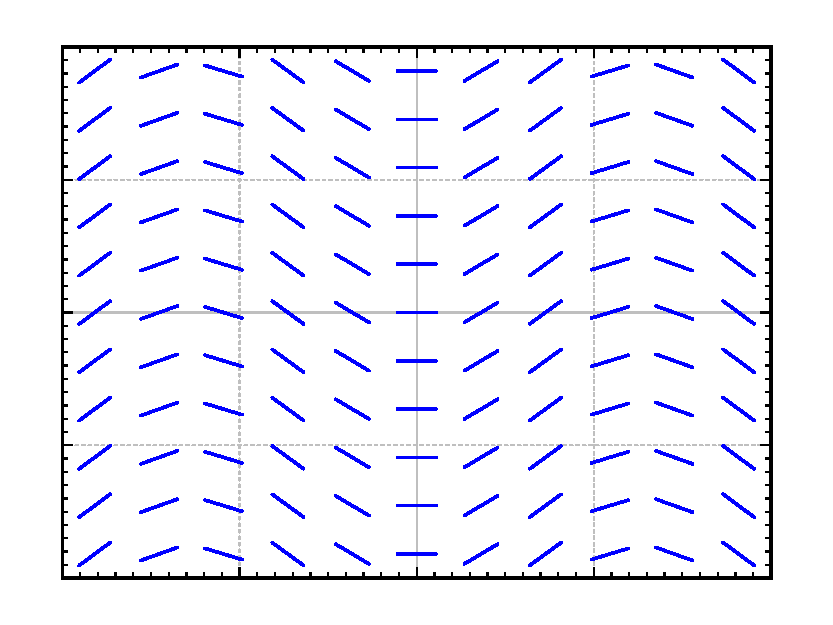
\includegraphics[width=1.75in]{figures/yprimesinxslope}}
\end{tasks}
\end{exercise}
\end{samepage}
\exsol{%
a) $y'=\cos y$, \quad
b) $y' = y\cos(x)$, \quad
c) $y'=\sin x$. \quad
Justification left to reader.
}

\begin{exercise}[tricky]
Suppose
\begin{equation*}
f(y) =
\begin{cases}
0 & \text{ if $y > 0$}, \\
1 & \text{ if $y \leq 0$} .
\end{cases}
\end{equation*}
Does $y' = f(y)$, $y(0) = 0$ have a continuously differentiable solution?  Does Picard apply?  Why, or why not?
\end{exercise}
\exsol{%
Picard does not apply as $f$ is not continuous at $y=0$.
The equation does not have a continuously differentiable solution.
Suppose it did. Notice that
$y'(0) = 1$.  By the first derivative test, $y(x) > 0$ for small positive $x$.
But then for those $x$ we would have $y'(x) = 0$, so clearly the derivative
cannot be continuous.
}

\begin{exercise}
Consider an equation of the form $y' = f(x)$ for some continuous function
$f$, and an initial condition $y(x_0) = y_0$.  Does a
solution exist for all $x$?  Why or why not?
\end{exercise}
\exsol{%
The solution is $y(x) = \int_{x_0}^x f(s) \,ds + y_0$, and this does indeed
exist for every $x$.
}

%%%%%%%%%%%%%%%%%%%%%%%%%%%%%%%%%%%%%%%%%%%%%%%%%%%%%%%%%%%%%%%%%%%%%%%%%%%%%%

\sectionnewpage
\section{Separable equations}
\label{separable:section}

\sectionnotes{1 lecture\EPref{, \S1.4 in \cite{EP}}\BDref{,
\S2.2 in \cite{BD}}}

When a differential equation is of the form
$y' = f(x)$,
we can just integrate:
$y = \int f(x) \,dx + C$. 
Unfortunately this method no longer works for the
general form of the equation
$y' = f(x,y)$.
Integrating both sides yields
\begin{equation*}
y = \int f(x,y) \,dx + C .
\end{equation*}
Notice the dependence on $y$ in the integral.

\subsection{Separable equations}

We say a differential equation is
\emph{\myindex{separable}}
if we can write it as
\begin{equation*}
y' = f(x)g(y) ,
\end{equation*}
for some functions $f(x)$ and $g(y)$.
Let us write the equation in the \myindex{Leibniz notation}
\begin{equation*}
\frac{dy}{dx} = f(x)g(y) .
\end{equation*}
Then we rewrite the equation as
\begin{equation*}
\frac{dy}{g(y)} = f(x) \,dx .
\end{equation*}
Both sides look like something we can integrate.  We obtain
\begin{equation*}
\int \frac{dy}{g(y)} = \int f(x) \,dx + C .
\end{equation*}
If we can find closed form expressions
for these two integrals, we can, perhaps, solve for $y$.

\begin{example} \label{example:yprimeisxy}
Take the equation
\begin{equation*}
y' = xy .
\end{equation*}
Note that $y=0$ is a solution.  We will remember that fact and
assume $y \not =0$ from now on, so that we can divide by $y$.
Write the equation as $\frac{dy}{dx} = xy$. Then
\begin{equation*}
\int \frac{dy}{y} = \int x\,dx + C .
\end{equation*}
We compute the antiderivatives to get
\begin{equation*}
\ln \, \lvert y\rvert = \frac{x^2}{2} + C ,
\end{equation*}
or
\begin{equation*}
\lvert y \rvert = e^{\frac{x^2}{2} + C} = e^{\frac{x^2}{2}} e^C = D e^{\frac{x^2}{2}} ,
\end{equation*}
where $D > 0$ is some constant.  Because $y=0$ is also a solution and because
of the absolute value we can write:
\begin{equation*}
y = D e^{\frac{x^2}{2}} ,
\end{equation*}
for any number $D$ (including zero or negative).

We check:
\begin{equation*}
y' = D x e^{\frac{x^2}{2}} = x \left( D e^{\frac{x^2}{2}} \right) = xy .
\end{equation*}
Yay!
\end{example}

We should be a little bit more careful with this method.  You may be worried 
that we 
integrated in two different variables.
We seemingly did
a different operation to each side.  Let us work through this method more
rigorously.  Take
\begin{equation*}
\frac{dy}{dx} = f(x)g(y) .
\end{equation*}
We rewrite the equation as follows.
Note that $y = y(x)$ is a function of $x$ and so is
$\frac{dy}{dx}$!
\begin{equation*}
\frac{1}{g(y)}\,\frac{dy}{dx} = f(x) .
\end{equation*}
We integrate both sides with respect to $x$:
\begin{equation*}
\int \frac{1}{g(y)}\,\frac{dy}{dx} \,dx = \int f(x) \,dx + C .
\end{equation*}
We use the change of variables formula (substitution) on the left hand side:
\begin{equation*}
\int \frac{1}{g(y)}\,dy = \int f(x) \,dx + C .
\end{equation*}
And we are done.

\subsection{Implicit solutions}

We sometimes get stuck even if we can do the
integration.  Consider the separable equation
\begin{equation*}
y' = \frac{xy}{y^2+1} .
\end{equation*}
We separate variables,
\begin{equation*}
\frac{y^2+1}{y}\,dy = \left(y+\frac{1}{y}\right)\,dy = x\,dx .
\end{equation*}
We integrate to get
\begin{equation*}
\frac{y^2}{2} + \ln \, \lvert y \rvert = \frac{x^2}{2} + C ,
\end{equation*}
or perhaps the easier looking expression (where $D = 2C$)
\begin{equation*}
y^2 + 2 \ln \, \lvert y\rvert = x^2 + D .
\end{equation*}
It is not easy to find the solution explicitly as it is hard to solve
for $y$.  We, therefore, leave the solution in this form and call
it an
\emph{\myindex{implicit solution}}.
It is still
easy to check that an implicit solution satisfies the differential
equation.  In this case, we differentiate with respect to $x$, and remember
that $y$ is a function of $x$,
to get
\begin{equation*}
y'\left(2y + \frac{2}{y}\right) = 2x .
\end{equation*}
Multiply both sides by $y$ and divide by $2(y^2+1)$ and you will
get exactly the differential equation.  We leave this computation to the
reader.

If you have an implicit solution, and
you want to compute values
for $y$, you might have to be tricky.  You might get multiple solutions $y$
for each $x$, so you have to pick one.  Sometimes you can
graph $x$ as a function of $y$, and then flip your paper.
Sometimes you have to do more.

Computers are also good at some of these tricks.
More advanced mathematical software usually has some
way of plotting solutions to implicit equations.
For example, for $C=0$ if you plot all the points $(x,y)$ that
are solutions to $y^2+2\ln|y|=x^2$,
you find the two curves in \figurevref{implicitsols:fig}.  This is not quite
a graph of a function. For each $x$ there are two choices of $y$.
To find a function you would have to pick one of these two curves.
You pick the one that satisfies your initial condition if you have one.
For example, the top curve satisfies the condition $y(1)=1$.
So for each $C$ we really got two solutions.
As you can see, computing values from an implicit solution can be somewhat
tricky.  But sometimes, an implicit solution is the best we can do.

\begin{myfig}
\capstart
\diffyincludegraphics{width=3in}{width=4.5in}{implicitsols}
\caption{The implicit solution $y^2+2\ln|y|=x^2$ to $y'=\frac{xy}{y^2+1}$.\label{implicitsols:fig}}
\end{myfig}


The equation above also has the solution $y=0$.
So the general solution is 
\begin{equation*}
y^2 + 2 \ln \, \lvert y \rvert = x^2 + C, \qquad \text{and} \qquad y=0.
\end{equation*}
These outlying solutions
such as $y=0$
are sometimes called \emph{singular solutions\index{singular solution}}.

\subsection{Examples of separable equations}

\begin{example}
Solve $x^2y' = 1 - x^2+y^2 - x^2y^2$, $y(1) = 0$.

Factor the right-hand side
\begin{equation*}
x^2y' = (1 - x^2)(1+y^2) .
\end{equation*}
Separate variables, integrate, and solve for $y$:
\begin{align*}
\frac{y'}{1+y^2} & = \frac{1 - x^2}{x^2} , \\
\frac{y'}{1+y^2} & = \frac{1}{x^2} - 1 , \\
\operatorname{arctan} (y) & = \frac{-1}{x} - x + C , \\
y & = \tan \left(\frac{-1}{x} - x + C\right) .
\end{align*}
Solve for the initial condition, $0 = \tan(-2+C)$ to get $C=2$ (or $C = 2 +
\pi$, or $C = 2 + 2\pi$, etc.).  The particular solution we seek is, therefore,
\begin{equation*}
y = \tan \left(\frac{-1}{x} - x + 2 \right) .
\end{equation*}
\end{example}

\begin{example} \label{sep:coffeeexample}
Bob made a cup of coffee, and
Bob likes to drink coffee only once reaches 60 degrees Celsius and will not burn him.
Initially at time $t=0$ minutes,
Bob measured the temperature and the coffee was 89 degrees Celsius.
One minute later, Bob measured the coffee again and it had 85 degrees.
The temperature of the room (the ambient temperature) is 22 degrees.
When should Bob start drinking?

Let $T$ be the temperature of the coffee in degrees Celsius, and let $A$ be
the ambient (room) temperature, also in degrees Celsius.
\myindex{Newton's law of cooling} states that the rate at which the
temperature of the coffee is changing
is proportional to the difference between the
ambient temperature and the temperature of the coffee.  That is,
\begin{equation*}
\frac{dT}{dt} = k(A-T) ,
\end{equation*}
for some positive constant $k$.
For our setup $A=22$, $T(0) = 89$, $T(1) = 85$.
We separate variables and integrate (let $C$ and $D$ denote arbitrary
constants):
\begin{align*}
\frac{1}{T-A} \, \frac{dT}{dt} & = -k , \\
\ln (T-A) &= -kt + C , \qquad \text{(note that } T-A > 0 \text{)} \\
T-A &= D\, e^{-kt} ,  \\
T &= A + D\, e^{-kt} .
\end{align*}
That is,
$T = 22 + D\, e^{-kt}$.  We plug in the first condition: $89 = T(0) = 22 +
D$,
and hence $D = 67$.  So
$T = 22 + 67\, e^{-kt}$.  The second condition says $85 = T(1) = 
22 + 67\, e^{-k}$.  Solving for $k$ we get
$k = - \ln \frac{85-22}{67} \approx 0.0616$.  Now we solve for the time $t$
that gives us a temperature of 60 degrees.  Namely, we solve
\begin{equation*}
60 = 22 + 67 e^{-0.0616t}
\end{equation*}
to get
$t = - \frac{\ln \frac{60-22}{67}}{0.0616} \approx 9.21$ minutes.  So Bob can
begin to drink the coffee at just over 9 minutes from the time Bob made
it.  That is probably about the amount of time it took us to calculate how long
it would take.  See \figurevref{sintro:coffeefig}.
\begin{myfig}
\capstart
%original files coffeefig-1 coffeefig-2
\diffyincludegraphics{width=6.24in}{width=9in}{coffeefig-1-2}
\caption{Graphs of the coffee temperature function $T(t)$.
On the left, horizontal
lines are drawn at temperatures 60, 85, and 89.  Vertical lines
are drawn at $t=1$ and $t=9.21$.  Notice that the
temperature of the coffee hits 85 at $t=1$, and 60 at
$t \approx 9.21$.  On the right, the graph is over a longer period of time,
with a horizontal line at the ambient temperature 22.\label{sintro:coffeefig}}
\end{myfig}
\end{example}

\begin{example}
Find the general solution to $y' = \frac{-xy^2}{3}$ (including singular
solutions).

First note that $y=0$ is a solution (a singular solution).
Now assume that $y \not= 0$.
\begin{align*}
\frac{-3}{y^2} y' & = x , \displaybreak[0]\\
\frac{3}{y} & = \frac{x^2}{2} + C , \displaybreak[0]\\
y & = \frac{3}{\nicefrac{x^2}{2} + C}
= \frac{6}{x^2 + 2C}.
\end{align*}
So the general solution is
\begin{equation*}
y = \frac{6}{x^2 + 2C} \qquad \text{and} \qquad y=0 .
\end{equation*}
\end{example}

\subsection{Exercises}

\begin{exercise}
Solve $y' = \nicefrac{x}{y}$.
\end{exercise}

\begin{exercise}
Solve $y' = x^2y$.
\end{exercise}

\begin{exercise}
Solve $\dfrac{dx}{dt} = (x^2-1)\,t$, for $x(0) = 0$.
\end{exercise}

\begin{exercise}
Solve $\dfrac{dx}{dt} = x\,\sin(t)$, for $x(0) = 1$.
\end{exercise}

\begin{exercise}
Solve $\dfrac{dy}{dx} = xy+x+y+1$.  Hint: Factor the right-hand side.
\end{exercise}

\begin{exercise}
Solve $xy' = y + 2x^2 y$, where $y(1) = 1$.
\end{exercise}

\begin{exercise}
Solve $\dfrac{dy}{dx} = \dfrac{y^2+1}{x^2+1}$, for $y(0) = 1$.
\end{exercise}

\begin{exercise}
Find an implicit solution for
$\dfrac{dy}{dx} = \dfrac{x^2+1}{y^2+1}$, for $y(0) = 1$.
\end{exercise}

\begin{exercise}
Find an explicit solution for $y' = xe^{-y}$, $y(0)=1$.
\end{exercise}

\begin{exercise}
Find an explicit solution for $xy' = e^{-y}$, for $y(1)=1$.
\end{exercise}

\begin{exercise}
Find an explicit solution for $y' = ye^{-x^2}$, $y(0)=1$.  It is alright to
leave a definite integral in your answer.
\end{exercise}

\begin{exercise}
Suppose a cup of coffee is at 100 degrees Celsius at time $t=0$,
it is at 70 degrees at $t=10$ minutes, and it is at 50 degrees at $t=20$
minutes.  Compute the ambient temperature.
\end{exercise}

\setcounter{exercise}{100}

\begin{exercise}
Solve $y'=2xy$.
\end{exercise}
\exsol{%
$y = Ce^{x^2}$
}

\begin{exercise}
Solve $x'=3xt^2-3t^2$, $x(0)=2$.
\end{exercise}
\exsol{%
$x = e^{t^3}+1$
}

\begin{exercise}
Find an implicit solution for
$x'=\frac{1}{3x^2+1}$, $x(0)=1$.
\end{exercise}
\exsol{%
$x^3+x=t+2$
}

\begin{exercise}
Find an explicit solution to $x y' = y^2$, $y(1) = 1$.
\end{exercise}
\exsol{%
$y = \frac{1}{1-\ln x}$
}

\begin{exercise}
Find an implicit solution to $y' = \frac{\sin(x)}{\cos(y)}$.
\end{exercise}
\exsol{%
$\sin(y) = -\cos(x) + C$
}

\begin{exercise}
Take \exampleref{sep:coffeeexample} with the same numbers: 89 degrees at
$t=0$, 85 degrees at $t=1$, and ambient temperature
of 22 degrees.  Suppose these temperatures were measured with precision of
$\pm 0.5$ degrees.  Given this imprecision, the time
it takes the coffee to cool to (exactly) 60 degrees is also only known in a
certain range.  Find this range.  Hint: Think about what kind of error makes
the cooling time longer and what shorter.
\end{exercise}
\exsol{%
The range is approximately 7.45 to 12.15 minutes.
}

\begin{exercise}
A population $x$ of rabbits on an island is modeled by
$x' = x- \bigl(\nicefrac{1}{1000} \bigr) x^2$, where the independent
variable is time in months.  At time $t=0$, there are 40 rabbits
on the island.
\begin{tasks}
\task Find the solution to the equation with the initial
condition.
\task
How many rabbits are on the island in 1 month, 5 months, 
10 months, 15 months (round to the nearest integer).
\end{tasks}
\end{exercise}
\exsol{%
a) $x = \frac{1000e^t}{e^t+24}$. \quad b) 102 rabbits after one month,
861 after 5 months, 999 after 10 months, 1000 after 15 months.
}

%%%%%%%%%%%%%%%%%%%%%%%%%%%%%%%%%%%%%%%%%%%%%%%%%%%%%%%%%%%%%%%%%%%%%%%%%%%%%%

\sectionnewpage
\section{Linear equations and the integrating factor}
\label{intfactor:section}

\sectionnotes{1 lecture\EPref{, \S1.5 in \cite{EP}}\BDref{,
\S2.1 in \cite{BD}}}

One of the most important types of equations we will learn how to solve are
the so-called
\emph{linear equations\index{linear equation}}.
In fact, the majority of the course is about linear
equations.  In this section we focus on the
\emph{\myindex{first order linear equation}}.
A first order equation is linear if we can put it
into the form:
\begin{equation} \label{lineq:eq1}
y' + p(x) y = f(x) .
\end{equation}
The word
\myquote{linear} means linear in $y$ and $y'$;
no higher powers nor functions of $y$ or $y'$ appear.
The dependence on $x$ can be more
complicated.

Solutions of linear equations have nice properties.  For example, the
solution exists wherever $p(x)$ and $f(x)$ are defined, and has the same
regularity (read: it is just as nice).  But most importantly for us right now,
there is a method for solving linear first order equations.

The trick is to rewrite the left-hand side
of \eqref{lineq:eq1} as a derivative of a product of $y$ with another
function.
To this end
we find a function $r(x)$ such that
\begin{equation*}
r(x) y' + r(x) p(x) y = \frac{d}{dx}\Bigl[ r(x) y \Bigr] .
\end{equation*}
This is the left-hand side of
\eqref{lineq:eq1} multiplied by $r(x)$.  So if we multiply \eqref{lineq:eq1} by
$r(x)$, we obtain
\begin{equation*}
\frac{d}{dx}\Bigl[ r(x) y \Bigr] = r(x)f(x) .
\end{equation*}
Now we integrate both sides.
The right-hand side does not depend on $y$ and the left-hand side
is written as a derivative of a function.  Afterwards, we solve for $y$.
The function $r(x)$ is called the \emph{\myindex{integrating factor}} and the
method is called the \emph{\myindex{integrating factor method}}.

We are looking for a function $r(x)$, such that if
we differentiate it, we get the same function back multiplied by $p(x)$.
That seems like a job for the exponential function!  Let
\begin{equation*}
r(x) = e^{\int p(x) \,dx} .
\end{equation*}
We compute:
\begin{align*}
y' + p(x) y &= f(x) , \\
e^{\int p(x) \,dx} y' + e^{\int p(x) \,dx} p(x) y & = e^{\int p(x) \,dx} f(x) , \\
\frac{d}{dx}\left[ e^{\int p(x) \,dx} y \right] & = e^{\int p(x) \,dx} f(x) , \\
e^{\int p(x) \,dx} y & = \int e^{\int p(x) \,dx} f(x) \,dx + C , \\
y & = e^{-\int p(x) \,dx} \left( \int e^{\int p(x) \,dx} f(x) \,dx + C \right) .
\end{align*}

Of course, to get a closed form formula for $y$,
we need to be able to find a
closed form formula for the integrals appearing above.

\begin{example}
Solve
\begin{equation*}
y' + 2xy = e^{x-x^2}, \qquad y(0) = -1 .
\end{equation*}

First note that $p(x) = 2x$ and $f(x) = e^{x-x^2}$.
The integrating factor is $r(x) = e^{\int p(x)\, dx} = e^{x^2}$.
We multiply both sides of the equation by $r(x)$ to get
\begin{align*}
e^{x^2} y' + 2xe^{x^2}y & = e^{x-x^2} e^{x^2} , \\
\frac{d}{dx} \left[ e^{x^2} y \right] &= e^x .
\end{align*}
We integrate
\begin{align*}
e^{x^2} y &= e^x +C , \\
y &= e^{x-x^2} + C e^{-x^2} .
\end{align*}
Next, we solve for the initial condition $-1 = y(0) = 1 + C$, so $C=-2$.
The solution is
\begin{equation*}
y = e^{x-x^2} - 2 e^{-x^2} .
\end{equation*}
\end{example}

Note that we do not care which antiderivative we take when computing
$e^{\int p(x) dx}$.  You can always add a constant of integration,
but those constants
will not matter in the end.

\begin{exercise}
Try it!  Add a constant of integration to the integral in
the integrating factor and show that the solution you get in the end is the
same as what we got above.
\end{exercise}

Advice: Do not try to remember the formula itself, that is way too
hard.  It is easier to remember the process and repeat it.

Since we cannot always evaluate the integrals in closed form, it is useful to
know how to write the solution in definite integral form.  A definite
integral is something that
you can plug into a computer or a calculator.  Suppose we are given
\begin{equation*}
y' + p(x) y = f(x) , \qquad y(x_0) = y_0 .
\end{equation*}
Look at the solution and write the integrals
as definite integrals.
\begin{equation} \label{lei:defsol}
\mybxbg{
~~
y(x) = e^{-\int_{x_0}^x p(s)\, ds} \left( \int_{x_0}^x e^{\int_{x_0}^t p(s)\, ds}
f(t) \,dt + y_0 \right).
~~
}
\end{equation}
You should
be careful to properly use dummy variables here.  If you now plug such a
formula into a
computer or a calculator, it will be happy to give you numerical answers.

\begin{exercise}
Check that $y(x_0) = y_0$ in formula \eqref{lei:defsol}.
\end{exercise}

\begin{exercise}
Write the solution of the following problem
as a definite integral, but try to simplify as far as you can.  You will not
be able to find the solution in closed form.
\begin{equation*}
y' + y = e^{x^2-x}, \qquad y(0) = 10 .
\end{equation*}
\end{exercise}

\begin{remark}
Before we move on, we should note some interesting properties of linear
equations.  First, for the linear initial value problem
$y' + p(x) y = f(x)$, $y(x_0) = y_0$,
there is always an explicit formula \eqref{lei:defsol} for the
solution.  Second, it follows
from the formula \eqref{lei:defsol} that if $p(x)$
and $f(x)$ are continuous on some interval $(a,b)$, then the 
solution $y(x)$ exists and is differentiable on $(a,b)$.  Compare
with the simple nonlinear example we have seen previously, $y'=y^2$,
and compare to \thmref{slope:picardthm}.
\end{remark}


\begin{example}
Let us discuss a common
simple application of linear equations.
This type of 
problem is used often in real life.
For example, linear equations are used in
figuring out the concentration of
chemicals in bodies of water (rivers and lakes).

\begin{mywrapfigsimp}{1.60in}{1.65in}
\noindent
\inputpdft{lin-tank}
\end{mywrapfigsimp}
A 100 liter tank contains 10 kilograms of salt dissolved in 60 liters of
water.  Solution of water and salt (brine) with concentration of 0.1
kilograms per
liter is flowing in at the rate of 5 liters a minute.  The solution
in the tank is well stirred and flows out at a rate of 3 liters a minute.
How much salt is in the tank when the tank is full?

Let us come up with the equation.  Let $x$ denote the kilograms of salt in the tank,
let $t$ denote the time in minutes.  For a small change $\Delta t$ in
time, the change in $x$ (denoted $\Delta x$) is approximately
\begin{equation*}
\Delta x \approx
(\text{rate in} \times \text{concentration in}) \Delta t - 
(\text{rate out} \times \text{concentration out}) \Delta t .
\end{equation*}
Dividing through by $\Delta t$ and
taking the limit $\Delta t \to 0$, we see that
\begin{equation*}
\frac{dx}{dt} =
(\text{rate in} \times \text{concentration in})  - 
(\text{rate out} \times \text{concentration out}) .
\end{equation*}
In our example,
\begin{align*}
\text{rate in} &= 5 , \\
\text{concentration in} &= 0.1 , \\
\text{rate out} &= 3 , \\
\text{concentration out} &= \frac{x}{\text{volume}} = \frac{x}{60+(5-3)t} .
\end{align*}
Our equation is, therefore,
\begin{equation*}
\frac{dx}{dt} =
(5 \times 0.1)  - 
\left(3 \frac{x}{60+2t}\right) .
\end{equation*}
Or in the form \eqref{lineq:eq1}
\begin{equation*}
\frac{dx}{dt} +
\frac{3}{60+2t} x
=
0.5 .
\end{equation*}

Let us solve.  The integrating factor is
\begin{equation*}
r(t) = \exp \left( \int \frac{3}{60+2t} dt  \right)
=
\exp \left( \frac{3}{2} \ln (60+2t) \right)
=
{(60+2t)}^{3/2} .
\end{equation*}
We multiply both sides of the equation to get
\begin{align*}
{(60+2t)}^{3/2} \frac{dx}{dt} +
{(60+2t)}^{3/2} \frac{3}{60+2t} x
& =
0.5{(60+2t)}^{3/2} ,\\
\frac{d}{dt}\left[
{(60+2t)}^{3/2} x \right]
& =
0.5{(60+2t)}^{3/2} ,\\
{(60+2t)}^{3/2} x
& =
\int 
0.5{(60+2t)}^{3/2}
dt
+C ,\\
 x
& =
{(60+2t)}^{-3/2} \int 
\frac{
{(60+2t)}^{3/2}
}{2}
dt
+C{(60+2t)}^{-3/2} ,\\
 x
& =
{(60+2t)}^{-3/2}
\frac{1}{10}{(60+2t)}^{5/2}
+C{(60+2t)}^{-3/2} ,\\
 x
& =
\frac{60+2t}{10}
+C{(60+2t)}^{-3/2} .
\end{align*}

%mbxSTARTIGNORE
\begin{mywrapfig}{3.25in}
\capstart
\diffyincludegraphics{width=3in}{width=4.5in}{linear-salt-graph}
\caption{Graph of the solution $x$ kilograms of salt in the tank at time
$t$.\label{linear-salt-graph:fig}}
\end{mywrapfig}
%mbxENDIGNORE
%
% Make sure to keep the above and the mbx figure below in sync!
%
To find $C$, note that at $t=0$, we have $x=10$.  That is,
\begin{equation*}
10 = x(0)
=
\frac{60}{10}
+C{(60)}^{-3/2}
=
6
+C{(60)}^{-3/2} ,
\end{equation*}
or
\begin{equation*}
C=4 ({60}^{3/2}) \approx 1859.03 .
\end{equation*}

We know $5$ liters per minute are flowing in and $3$ liters per minute are flowing out,
so the volume is increasing by $2$ liters a minute.
So the tank is
full when $60+2t = 100$, or when $t=20$.
We are interested in the value of $x$ when the tank is full,
that is we want to compute $x(20)$:
\begin{equation*}
\begin{split}
x(20) & = 
\frac{60+40}{10}
+C{(60+40)}^{-3/2}
\\
& \approx
10
+1859.03 {(100)}^{-3/2}
\approx
11.86 .
\end{split}
\end{equation*}
See \figurevref{linear-salt-graph:fig} for the graph of $x$ over $t$.

The concentration when the tank is full is approximately
$\nicefrac{11.86}{100} = \unitfrac[0.1186]{kg}{liter}$, and we started
with $\nicefrac{1}{6}$ or \unitfrac[0.167]{kg}{liter}.
%mbxlatex \begin{myfig}
%mbxlatex \capstart
%mbxlatex \diffyincludegraphics{width=3in}{width=4.5in}{linear-salt-graph}
%mbxlatex \caption{Graph of the solution $x$ kilograms of salt in the tank at time
%mbxlatex $t$.\label{linear-salt-graph:fig}}
%mbxlatex \end{myfig}
\end{example}

\subsection{Exercises}

In the exercises, feel free to leave answer as a definite integral if a
closed form solution cannot be found.  If you can find a closed form
solution, you should give that.

\begin{exercise}
Solve $y' + xy = x$.
\end{exercise}

\begin{exercise}
Solve $y' + 6y = e^x$.
\end{exercise}

\begin{exercise}
Solve $y' + 3x^2y = \sin(x) \, e^{-x^3}$, with $y(0) = 1$.
\end{exercise}

\begin{exercise}
Solve $y' + \cos (x) y = \cos(x)$.
\end{exercise}

\begin{exercise}
Solve $\frac{1}{x^2+1} \, y' + x y = 3$, with $y(0) = 0$.
\end{exercise}

\begin{exercise}
Suppose there are two lakes located on a stream.  Clean
water flows into the first lake,
then the water from the first lake flows into the second lake, and then
water from the second lake flows further downstream.
The in and out flow from each lake is 500 liters per hour.
The first lake contains 100 thousand liters of water and the
second lake contains 200 thousand liters of water.
A truck with \unit[500]{kg} of toxic substance
crashes into the first lake.  Assume that the water is being continually
mixed perfectly by the stream.
\begin{tasks}
\task Find the concentration of toxic substance
as a function of time in both lakes.
\task When will the
concentration in the first lake be below \unit[0.001]{kg} per liter?
\task When will the
concentration in the second lake be maximal?
\end{tasks}
\end{exercise}

\begin{exercise}
\myindex{Newton's law of cooling} states that $\frac{dx}{dt} = -k(x-A)$ where
$x$ is the temperature, $t$ is time, $A$ is the ambient temperature,
and $k > 0$ is a constant.
Suppose that $A = A_0 \cos (\omega t)$ for some constants $A_0$ and $\omega$.
That is, the ambient temperature oscillates (for example night and day
temperatures).
\begin{tasks}
\task Find the general solution.
\task In the long term, will the
initial conditions make much of a difference?  Why or why not?
\end{tasks}
\end{exercise}

\begin{exercise}
Initially 5 grams of salt are dissolved in 20 liters of water.  Brine
with concentration of salt 2 grams of salt per liter is added at a rate
of 3 liters a minute.  The tank is mixed well and is drained at 3 liters
a minute.  How long does the process have to continue until there are 20 grams
of salt in the tank?
\end{exercise}

\begin{exercise}
Initially a tank contains 10 liters of pure water.
Brine of unknown (but constant) concentration
of salt is flowing in at 1 liter per minute.
The water is mixed well and drained at 1 liter per minute.
In 20 minutes there are 15 grams of salt in the tank.  What is the
concentration of salt in the incoming brine?
\end{exercise}

\setcounter{exercise}{100}

\begin{exercise}
Solve $y'+3 x^2 y = x^2$.
\end{exercise}
\exsol{%
$y = C e^{-x^3} + \nicefrac{1}{3}$
}

\begin{exercise}
Solve $y'+ 2\sin(2x) y = 2\sin(2x)$, $y(\nicefrac{\pi}{2}) = 3$.
\end{exercise}
\exsol{%
$y = 2 e^{\cos(2x)+1} + 1$
}

\begin{exercise}
Suppose a water tank is being pumped out at \unitfrac[3]{L}{min}.  The
water tank starts at \unit[10]{L} of clean water.
Water with
toxic substance is flowing into the tank at \unitfrac[2]{L}{min},
with concentration \unitfrac[$20t$]{g}{L} at time $t$.
When the tank is half empty, how many grams of toxic substance are in the
tank (assuming perfect mixing)?
\end{exercise}
\exsol{%
$250$ grams
}

\begin{exercise}
There is bacteria on a plate and a toxic substance is being added that slows
down the rate of growth of the bacteria.
That is,
suppose that $\frac{dP}{dt} = (2-0.1\,t)P$.  If $P(0) = 1000$, find
the population at $t=5$.
\end{exercise}
\exsol{%
$P(5) = 1000 e^{2 \times 5 - 0.05 \times {5}^2} = 1000 e^{8.75} \approx
6.31 \times {10}^6$
}

\begin{exercise}
A cylindrical water tank has water flowing in at $I$ cubic meters
per second.
Let $A$ be the area of the cross section of the tank in square meters.
Suppose water is
flowing out from the bottom of the tank at a rate proportional to the height of
the water level.  Set up the differential equation for $h$, the height of the
water, introducing and naming
constants that you need.  You should also give the units for your constants.
\end{exercise}
\exsol{%
$Ah' = I - kh$, where $k$ is a constant with units $\unitfrac{m^2}{s}$.
}

%%%%%%%%%%%%%%%%%%%%%%%%%%%%%%%%%%%%%%%%%%%%%%%%%%%%%%%%%%%%%%%%%%%%%%%%%%%%%%

\sectionnewpage
\section{Substitution}
\label{substitution:section}

\sectionnotes{1 lecture, can safely be skipped\EPref{, \S1.6 in \cite{EP}}\BDref{, not in
\cite{BD}}}

Just as when solving integrals, one method to try is to change variables to
end up with a simpler equation to solve.

\subsection{Substitution}

The equation
\begin{equation*}
y' = {(x-y+1)}^2 
\end{equation*}
is neither separable nor linear.  What can we do?
How about trying to change variables, so that in the new variables the
equation is simpler.  We use another variable $v$, which we treat as
a function of $x$.  We try
\begin{equation*}
v = x-y+1 .
\end{equation*}
We need to figure out
$y'$ in terms of $v'$, $v$ and $x$.  We differentiate (in $x$) to
obtain $v' = 1 - y'$.  So $y' = 1-v'$.  We plug this into the equation to get
\begin{equation*}
1-v' = v^2 .
\end{equation*}
In other words, $v' = 1-v^2$.  Such an equation we know how to solve by
separating variables:
\begin{equation*}
\frac{1}{1-v^2} \,dv = dx .
\end{equation*}
So
\begin{equation*}
\frac{1}{2} \ln \left\lvert  \frac{v+1}{v-1} \right\rvert = x + C ,
\qquad \text{or} \qquad
\left\lvert \frac{v+1}{v-1} \right\rvert = e^{2x + 2C} ,
\qquad \text{or} \qquad
\frac{v+1}{v-1} = D e^{2x} ,
\end{equation*}
for some constant $D$.
Note that $v=1$ and $v=-1$ are also solutions.

Now we need to \myquote{unsubstitute} to obtain
\begin{equation*}
\frac{x-y+2}{x-y} = D e^{2x} ,
\end{equation*}
and also the two solutions $x-y+1=1$ or $y=x$, and $x-y+1=-1$ or $y=x+2$.
We solve the first equation for $y$.
\begin{align*}
x-y+2 &= (x-y)D e^{2x} , \\
x-y+2 &= Dx e^{2x}-yD e^{2x} , \\
-y + yD e^{2x} &= Dx e^{2x} - x - 2 , \displaybreak[0]\\
y\,(-1+ D e^{2x}) &= Dx e^{2x} - x - 2 , \displaybreak[0]\\
y  &= \frac{Dx e^{2x} - x - 2}{D e^{2x}-1} .
\end{align*}
Note that $D=0$ gives $y=x+2$, but no value of $D$ gives the solution $y=x$.

\medskip

Substitution in differential equations is applied in much the same way that
it is applied in calculus.  You guess.  Several different substitutions might
work.  There are some general patterns to look for.  We summarize a few
of these in a table.

\begin{center}
\begin{tabular}{@{}ll@{}}
\toprule
When you see & Try substituting \\
\midrule
$yy'$ & $v=y^2$ \\
$y^2y'$ & $v=y^3$ \\
$(\cos y)y'$ & $v=\sin y$ \\
$(\sin y)y'$ & $v=\cos y$ \\
$e^y y'$ & $v=e^y$ \\ \bottomrule
\end{tabular}
\end{center}

Usually you try to substitute in the \myquote{most complicated} part of the
equation with the hopes of simplifying it.  The table above is just a rule
of thumb.  You might have to modify your guesses.  If a substitution
does not work (it does not make the equation any simpler), try a different one.

\subsection{Bernoulli equations}

There are some forms of equations where there is a
general rule for substitution that always works.
One such example is the so-called
\emph{\myindex{Bernoulli equation}}%
\footnote{There are several things called Bernoulli equations, this is just one
of them.  The Bernoullis were a prominent Swiss family of mathematicians.  These
particular equations are named for
\href{https://en.wikipedia.org/wiki/Jacob_Bernoulli}{Jacob Bernoulli} (1654--1705).}:
\begin{equation*}
y' + p(x)y = q(x)y^n .
\end{equation*}
This equation
looks a lot like a linear equation except for the $y^n$.  If $n=0$ or
$n=1$, then the equation is linear and we can solve it.  Otherwise,
the substitution $v=y^{1-n}$ transforms the 
Bernoulli equation into a linear equation.  Note that $n$
need not be an integer.

\begin{example}
Solve
\begin{equation*}
xy'+ y(x+1)+xy^5 = 0, \qquad y(1)=1 .
\end{equation*}
The equation is a Bernoulli equation, $p(x) = (x+1)/x$ and $q(x) = -1$.
We substitute
\begin{equation*}
v=y^{1-5} = y^{-4}, \qquad
v' = -4 y^{-5} y' .
\end{equation*}
In other words, $\left( \nicefrac{-1}{4} \right) y^5 v' = y'$.  So
\begin{align*}
xy'+ y(x+1)+xy^5 & = 0 , \\
\frac{-xy^5}{4} v'+ y(x+1)+xy^5 & = 0 , \displaybreak[0]\\
\frac{-x}{4} v'+ y^{-4}(x+1)+x & = 0 , \displaybreak[0]\\
\frac{-x}{4} v'+ v(x+1)+x & = 0 ,
\end{align*}
and finally
\begin{equation*}
v'- \frac{4(x+1)}{x} v  = 4 .
\end{equation*}
The equation is now linear.
We can use the integrating factor method.  In particular, we
use formula \eqref{lei:defsol}.  We assume that $x > 0$
so $\lvert x \rvert = x$.  This assumption is OK\@, as our initial condition is
at $x=1 > 0$.  Let us compute the integrating factor.  Here $p(s)$ from formula
\eqref{lei:defsol} is $\frac{-4(s+1)}{s}$.
\begin{align*}
e^{\int_1^x p(s)\,ds} & = \exp \left( \int_1^x \frac{-4(s+1)}{s} \,ds \right) =
e^{-4x-4\ln(x)+4} = 
e^{-4x+4} x^{-4}
=
\frac{e^{-4x+4}}{x^4} , \\
e^{-\int_1^x p(s)\,ds} & =
e^{4x+4\ln(x)-4} = 
e^{4x-4} x^4 .
\end{align*}
We now plug in to \eqref{lei:defsol}
\begin{equation*}
\begin{split}
v(x) & =
e^{-\int_{1}^x p(s)\, ds} \left( \int_{1}^x e^{\int_{1}^t p(s)\, ds} 4 \,dt
+ 1 \right) \\
& =
e^{4x-4} x^4
\left( \int_{1}^x 4 \frac{e^{-4t+4}}{t^4} \,dt
+ 1 \right) .
\end{split}
\end{equation*}
The integral in this expression is not possible to find in closed
form.  As we said before, it is perfectly fine to have a
definite integral in our solution.  Now \myquote{unsubstitute}
\begin{align*}
 y^{-4} &= e^{4x-4}x^4 \left( 4 \int_1^x \frac{e^{-4t+4}}{t^4} \,dt + 1\right) , \\
 y &= \frac{e^{-x+1}}{x {\left( 4 \int_1^x \frac{e^{-4t+4}}{t^4} \,dt +
1\right)}^{1/4}} .
\end{align*}
\end{example}

\subsection{Homogeneous equations}

Another type of equations we can solve by substitution are the 
so-called \emph{homogeneous equations\index{homogeneous equation}}.
Suppose that we can write the differential equation as
\begin{equation*}
y' = F\left(\frac{y}{x}\right) .
\end{equation*}
Here we try the substitutions
\begin{equation*}
v = \frac{y}{x} \qquad \text{and therefore} \qquad y' = v + x v' .
\end{equation*}
We note that the equation is transformed into
\begin{equation*}
v+ xv' = F(v) \qquad \text{or} \qquad xv' = F(v)-v 
\qquad \text{or} \qquad \frac{v'}{F(v)-v} = \frac{1}{x} .
\end{equation*}
Hence an implicit solution is
\begin{equation*}
\int \frac{1}{F(v)-v} \,dv = \ln \, \lvert x \rvert + C .
\end{equation*}
Clearly this solution does not work when $x = 0$ (we would, afterall,
divide by zero in $\nicefrac{y}{x}$).  So we will either assume $x > 0$
or $x < 0$ depending on the initial condition.

\begin{example}
Solve 
\begin{equation*}
x^2y' = y^2+xy, \qquad y(1)=1.
\end{equation*}

We put the equation into
the form $y'= {\left(\nicefrac{y}{x}\right)}^2+\nicefrac{y}{x}$,
that is, $F(v) = v^2+v$.
As the initial condition is for a positive $x$ value,
we will assume $x > 0$.
We substitute $v=\nicefrac{y}{x}$ to get
the separable equation
\begin{equation*}
xv' = v^2+v-v = v^2 ,
\end{equation*}
which has a solution
\begin{align*}
\int \frac{1}{v^2} \,dv &= \ln \, \lvert x \rvert + C , \\
\frac{-1}{v} &= \ln  x + C , \\
v &= \frac{-1}{\ln  x  + C} .
\end{align*}
We unsubstitute
\begin{equation*}
\frac{y}{x} = \frac{-1}{\ln  x  + C} ,
\qquad
\text{or}
\qquad
y = \frac{-x}{\ln  x  + C} .
\end{equation*}
We want $y(1)=1$, so 
\begin{equation*}
1 = y(1) = \frac{-1}{\ln  1 + C} = \frac{-1}{C} .
\end{equation*}
Thus $C = -1$ and
the solution we are looking for is
\begin{equation*}
y = \frac{-x}{\ln  x  -1} .
\end{equation*}
\end{example}

\subsection{Exercises}

Hint: Answers need not always be in closed form.

\begin{exercise}
Solve
$y'+ y(x^2-1)+xy^6 = 0$, with $y(1)=1$.
\end{exercise}

\begin{exercise}
Solve $2yy' + 1 = y^2 + x$, with $y(0)=1$.
\end{exercise}

\begin{exercise}
Solve $y' + xy = y^4$, with $y(0)=1$.
\end{exercise}

\begin{exercise}
Solve $yy' + x = \sqrt{x^2 + y^2}$.
\end{exercise}

\begin{exercise}
Solve $y' = {(x+y-1)}^2$.
\end{exercise}

\begin{exercise}
Solve $y' = \frac{x^2-y^2}{x y}$, with $y(1) = 2$.
\end{exercise}

\setcounter{exercise}{100}

\begin{exercise}
Solve $xy'+y+y^2 = 0$, $y(1)=2$.
\end{exercise}
\exsol{%
$y = \frac{2}{3x-2}$
}

\begin{exercise}
Solve $xy'+y +x = 0$, $y(1)=1$.
\end{exercise}
\exsol{%
$y = \frac{3-x^2}{2 x}$
}

\begin{exercise}
Solve $y^2y' = y^3-3x$, $y(0)=2$.
\end{exercise}
\exsol{%
$y = {\bigl(7 e^{3x} + 3x + 1 \bigr)}^{1/3}$
}

\begin{exercise}
Solve $2yy' = e^{y^2-x^2} + 2x$.
\end{exercise}
\exsol{%
$y = \pm\sqrt{x^2-\ln(C-x)}$
}

%%%%%%%%%%%%%%%%%%%%%%%%%%%%%%%%%%%%%%%%%%%%%%%%%%%%%%%%%%%%%%%%%%%%%%%%%%%%%%

\sectionnewpage
\section{Autonomous equations}
\label{auteq:section}

\sectionnotes{1 lecture\EPref{, \S2.2 in \cite{EP}}\BDref{,
\S2.5 in \cite{BD}}}

Consider
problems of the form
\begin{equation*}
\frac{dx}{dt} = f(x) ,
\end{equation*}
where the derivative of solutions depends only on $x$ (the dependent
variable).  Such equations are called \emph{autonomous
equations\index{autonomous equation}}.  If we think
of $t$ as time, the naming comes from the fact that the equation is
independent of time.

We return to the cooling coffee problem
(\exampleref{sep:coffeeexample}).
\myindex{Newton's law of cooling}
says
\begin{equation*}
\frac{dx}{dt} = k (A-x) ,
\end{equation*}
where $x$ is the temperature, $t$ is time, $k$ is some positive constant,
and $A$ is
the ambient temperature.  See \figurevref{2.2:coffeefig} for an example
with $k=0.3$ and $A=5$.

Note the solution $x=A$ (in the figure $x=5$).
We call these constant solutions the
\emph{equilibrium solutions}\index{equilibrium solution}.
The points on the $x$-axis where $f(x) = 0$ are called
\emph{critical points\index{critical point}}.  The point
$x=A$ is a critical point.  In fact, each
critical point corresponds to an equilibrium solution.
Note also, by looking at the graph, that the solution $x=A$ is
\myquote{stable} in
that small perturbations in $x$ do not lead to substantially different
solutions as $t$ grows.
If we change the initial condition a little bit, then as 
$t \to \infty$ we get $x(t) \to A$.  We call such a critical point
\emph{stable}\index{stable critical point}.
In this simple example it turns out that all solutions in fact go to $A$
as $t \to \infty$.  If a critical point is not stable, we say it is
\emph{unstable}\index{unstable critical point}.

\begin{myfig}
\parbox[t]{3.0in}{
 \capstart
 \diffyincludegraphics{width=2.93in}{width=4.5in}{2-2-coffee}
 \caption{The slope field and some solutions of
 $x' = 0.3\,(5-x)$.\label{2.2:coffeefig}}
 %$dx/dt = -0.3*(x-5)$, $t: [0,20], x: [-10,10]$, plot solutions for
 %$t=0$, $x=10$, $x=5$, $x=0$, $x=-5$, $x=-10$.
}
\quad
\parbox[t]{3.0in}{
 \capstart
 \diffyincludegraphics{width=3in}{width=4.5in}{2-2-logistic}
 \caption{The slope field and some solutions of
 $x' = 0.1\,x\,(5-x)$.\label{2.2:logisticfig}}
}
\end{myfig}

\medskip

Consider now the \emph{\myindex{logistic equation}}
\begin{equation*}
\frac{dx}{dt} = kx(M-x) ,
\end{equation*}
for some positive $k$ and $M$.  This equation is commonly used to model
population if we know the limiting population $M$, that is the maximum
sustainable population.  The logistic equation leads to 
less catastrophic
predictions on world population than $x'=kx$.  In the real world there is no
such thing as negative population, but we will still consider negative $x$ for
the purposes of the math.

See \figurevref{2.2:logisticfig} for an example, $x' = 0.1 x(5-x)$.
There are two critical points, $x=0$ and $x=5$.  The critical point
at $x=5$ is stable, while the critical point at $x=0$ is
unstable.
It is not necessary to find the exact solutions to understand their long
term behavior, that is, behavior as time goes to infinity.
From the slope field above of
$x' = 0.1 x(5-x)$, we 
see that
\begin{equation*}
\lim_{t\to \infty} x(t) = 
\begin{cases}
5 & \text{if } \; x(0) > 0 , \\
0 & \text{if } \; x(0) = 0 , \\
\text{DNE or } {-\infty} & \text{if } \; x(0) < 0 . \\
\end{cases}
\end{equation*}
Here DNE means \myquote{does not exist.}  From just looking at the slope field we
cannot quite decide what happens if $x(0) < 0$.  It could be that the
solution does not exist for $t$ all the way to $\infty$.
Think of the equation $x' = x^2$; we
have seen that solutions only exist for some finite period of time.  Same can happen
here.  In our example equation above it turns out that the
solution does not exist for all time, but to see that we would have to solve
the equation.  In any case, the solution does go to $-\infty$, but it may get
there rather quickly.


If we are interested only in the long term behavior of the solution, 
we would be doing unnecessary work if we solved the
equation exactly.
We could draw the slope field, but
it is easier to just look at the \emph{\myindex{phase diagram}} or
\emph{\myindex{phase portrait}}, which is a simple
way to visualize the behavior of
autonomous equations.  In this case there is one dependent variable $x$.
We draw the $x$-axis, we mark all the critical points,
and then we draw arrows in
between.  Since $x$ is the dependent variable we draw the axis vertically,
as it appears in the slope field diagrams above.
If $f(x) > 0$, we draw an up arrow.  If $f(x) < 0$, we draw 
a down arrow.
To figure this out, we could just plug in some $x$ between the critical
points, $f(x)$ will have the same sign at all $x$ between two critical
points as long $f(x)$ is continuous.
For example, $f(6) = -0.6 < 0$, so $f(x) < 0$ for $x > 5$,
and the arrow above $x=5$ is a down
arrow.  Next, $f(1) = 0.4 > 0$, so $f(x) > 0$ whenever $0 < x < 5$, and
the arrow points up.  Finally, $f(-1) = -0.6 < 0$ so $f(x) < 0$ when $x <
0$, and the arrow points down.

\begin{center}
\inputpdft{2-2-l-phasedia}
\end{center}

\pagebreak[0]
Armed with the phase diagram,
it is easy to sketch the solutions approximately:  As time $t$
moves from left to right,
the graph of a solution
goes up if the arrow is up, and it goes down if the arrow is down.

\begin{exercise}
Try sketching a few solutions simply from looking at the phase diagram.
Check with the preceding graphs if
you are getting the same type of curves.
\end{exercise}

\pagebreak[0]
Once we draw the phase diagram, we classify critical points
as stable or unstable\footnote{Unstable 
points with one of the
arrows pointing towards the critical point are sometimes called
\emph{semistable}\index{semistable critical point}.}.  
Since any mathematical model we cook up will only be an approximation
to the real world, unstable points are generally bad news.

\begin{center}
\inputpdft{2-2-ph-class}
\end{center}

We remark that you can figure out the arrows by plotting the graph $y=f(x)$.
However, in that case note that $x$ is then the dependent variable and will
be on the horizontal axis.

\medskip

Let us think about the logistic equation
with harvesting\index{logistic equation!with harvesting}\index{harvesting}.
Suppose an alien race really likes to
eat humans.  They keep a planet with humans and harvest the
humans at a rate of $h$ million humans per
year.  Suppose $x$
is the number of humans in millions on the planet and $t$ is time in years.
Let $M$ be the limiting
population when no harvesting is done.  The number $k > 0$ is a
constant depending
on how fast humans multiply.  Our equation becomes
\begin{equation*}
\frac{dx}{dt} = kx(M-x) - h .
\end{equation*}
We expand the right-hand side and set it to zero.
\begin{equation*}
kx(M-x) - h = -kx^2+kMx - h  = 0.
\end{equation*}
Solving for
the critical points,
let us call them $A$ and $B$, we get
\begin{equation*}
A = \frac{kM + \sqrt{{(kM)}^2 - 4hk}}{2k}, \qquad
B = \frac{kM - \sqrt{{(kM)}^2 - 4hk}}{2k} .
\end{equation*}

\begin{exercise}
Sketch a phase diagram for different possibilities.  Note
that these possibilities are $A > B$, or $A=B$, or $A$ and $B$ both complex
(i.e.\ no real solutions).  Hint: Fix some simple $k$ and $M$ and then vary
$h$.
\end{exercise}

For example, let $M=8$ and $k=0.1$.
When $h=1$, then $A$ and $B$ are distinct and positive.
See \figurevref{2.2:harv1} for the slope field.  As long as 
the population starts above $B$, which is approximately 1.55 million, then
the population will not die out, it will tend towards $A \approx
6.45$ million.  If ever a catastrophe happens and
the population drops below $B$,
humans will die out, and the fast food restaurant serving them will go out
of business.

\begin{myfig}
\parbox[t]{3.0in}{
 \capstart
 \diffyincludegraphics{width=3in}{width=4.5in}{2-2-logistic-h1}
 \caption{The slope field and some solutions of
 $x' = 0.1\,x\,(8-x)-1$.\label{2.2:harv1}}
}
\quad
\parbox[t]{3.0in}{
 \capstart
 \diffyincludegraphics{width=3in}{width=4.5in}{2-2-logistic-hc}
 \caption{The slope field and some solutions of
 $x' = 0.1\,x\,(8-x)-1.6$.\label{2.2:harvc}}
}
\end{myfig}

When $h = 1.6$, then $A=B=4$.  There is only one critical point and it is
unstable.  When the population starts above 4 million, it will tend towards
4 million.  However, if it ever drops below 4 million, perhaps a worse than
normal hurricane season one year, then humans will die out on the
planet.  This scenario is not one that we (as the human fast food proprietor) 
want to be in.  A small perturbation of the equilibrium state and we are out
of business.  There is no room for error.  See \figurevref{2.2:harvc}.

Finally, if we are harvesting at 2 million humans per year, there are no
critical points.
The population
will always plummet towards zero, no matter how well stocked the planet
starts.  See \figurevref{2.2:harv2}.

\begin{myfig}
\capstart
\diffyincludegraphics{width=3in}{width=4.5in}{2-2-logistic-h2}
\caption{The slope field and some solutions of
$x' = 0.1\,x\,(8-x)-2$.\label{2.2:harv2}}
\end{myfig}

%$dx/dt = 0.1*x*(8-x)-1$, $t: [0,20], x: [-5,10]$,

\subsection{Exercises}

\begin{samepage}
\begin{exercise}
Consider $x' = x^2$.
\begin{tasks}
\task Draw the phase diagram,
find the critical points, and mark them stable or unstable.
\task Sketch typical solutions of the equation.
\task Find $\displaystyle \lim_{t\to \infty} x(t)$ for the solution with the initial condition
$x(0) = -1$.
\end{tasks}
\end{exercise}
\end{samepage}

\begin{exercise}
Consider $x' = \sin x$.
\begin{tasks}
\task Draw the phase diagram for $-4\pi \leq x \leq 4\pi$.  On this interval
mark the critical points stable or unstable.
\task Sketch typical solutions of the equation.
\task Find $\displaystyle \lim_{t\to \infty} x(t)$ for the solution with the initial condition
$x(0) = 1$.
\end{tasks}
\end{exercise}

\begin{exercise}
Suppose $f(x)$ is positive for $0 < x < 1$, it is zero when $x=0$ and $x=1$,
and it is negative for all other $x$.
\begin{tasks}
\task Draw the phase diagram for $x' = f(x)$,
find the critical points, and mark them stable or unstable.
\task Sketch typical solutions of the equation.
\task Find $\displaystyle \lim_{t\to \infty} x(t)$ for the solution with the initial condition
$x(0) = 0.5$.
\end{tasks}
\end{exercise}

\begin{exercise}
Start with the logistic equation
$\frac{dx}{dt} = kx(M-x)$.
Suppose we modify our harvesting.  That is we will only harvest 
an amount proportional to current population.  In other words, we harvest $hx$
per unit of time
for some $h > 0$ (similar to earlier example with $h$ replaced with $hx$).
\begin{tasks}
\task Construct the differential equation. 
\task Show that if $kM > h$, then
the equation is still logistic.
\task What happens when $kM < h$?
\end{tasks}
\end{exercise}

\begin{exercise}
A disease is spreading through the country.  Let $x$ be the number of people
infected.  Let the constant $S$ be the number of people susceptible to
infection.  The infection rate $\frac{dx}{dt}$ is proportional to the product
of already infected people, $x$, and the number of susceptible but
uninfected people, $S-x$.
\begin{tasks}
\task Write down the differential equation.
\task Supposing $x(0) > 0$, that is, some people are infected at time $t=0$,
what is
$\displaystyle \lim_{t\to\infty} x(t)$.
\task Does the solution to part b) agree with your intuition?  Why or why not?
\end{tasks}
\end{exercise}


\setcounter{exercise}{100}

\begin{exercise}
\pagebreak[2]
Let $x'=(x-1)(x-2)x^2$.
\begin{tasks}
\task Sketch the phase diagram and find critical
points.
\task Classify the critical points.
\task If $x(0)=0.5$, then find $\displaystyle \lim_{t\to\infty} x(t)$.
\end{tasks}
\end{exercise}
\exsol{%
a) 0, 1, 2 are critical points.
\quad
b) $x=0$ is unstable (semistable), $x=1$ is stable, and $x=2$ is unstable.
\quad
c) 1
}

\begin{exercise}
Let $x'=e^{-x}$.
\begin{tasks}(2)
\task Find and classify all critical points.
\task Find $\displaystyle \lim_{t\to\infty} x(t)$ given any 
initial condition.
\end{tasks}
\end{exercise}
\exsol{%
a) There are no critical points.
\quad
b) $\infty$
}

\begin{exercise}
Assume that a population of fish in a lake satisfies
$\frac{dx}{dt} = kx(M-x)$.  Now suppose that fish are continually added
at $A$ fish per unit of time.
\begin{tasks}(2)
\task Find the differential equation for $x$.
\task What is the new limiting population?
\end{tasks}
\end{exercise}
\exsol{%
a) $\frac{dx}{dt} = kx(M-x)+A$
\quad
b) $\frac{kM + \sqrt{{(kM)}^2 + 4Ak}}{2k}$
}

\begin{exercise}
Suppose $\frac{dx}{dt} = (x-\alpha)(x-\beta)$ for two numbers $\alpha <
\beta$.
\begin{tasks}
\task Find the critical points, and classify them.
\end{tasks}
For b), c), d), find $\displaystyle \lim_{t\to\infty} x(t)$ based on
the phase diagram.
\begin{tasks}[resume](3)
\task $x(0) < \alpha$,
\task $\alpha < x(0) < \beta$,
\task $\beta < x(0)$.
\end{tasks}
\end{exercise}
\exsol{%
a) $\alpha$ is a stable critical point, $\beta$ is an unstable one.
\quad
b) $\alpha$, \quad c) $\alpha$, \quad d) $\infty$ or DNE\@.
}

%%%%%%%%%%%%%%%%%%%%%%%%%%%%%%%%%%%%%%%%%%%%%%%%%%%%%%%%%%%%%%%%%%%%%%%%%%%%%%

\sectionnewpage
\section{Numerical methods: Euler's method}
\label{numer:section}

\sectionnotes{1 lecture, can safely be skipped\EPref{, \S2.4 in \cite{EP}}\BDref{,
\S8.1 in \cite{BD}}}

%At this point it may be good to first try the
%Lab II\index{IODE software!Lab II} and/or Project II\index{IODE software!Project II} from the
%IODE website: \url{http://www.math.uiuc.edu/iode/}.
%
%\medskip

%You worked with Euler's method in the IODE lab, let us now go over this method
%to see what we've done.

Unless $f(x,y)$ is of a special form,
it is generally very hard
if not impossible to get a nice formula for the solution of the problem
\begin{equation*}
y' = f(x,y), \qquad y(x_0) = y_0 .
\end{equation*}

If the equation can be solved in closed form, we should do that.
But what if we have an equation that cannot be solved in closed form?
What if we want to find the value of the solution at some particular $x$?
Or perhaps we want to produce a graph of the solution to inspect the
behavior.  In this section we will learn about the basics of numerical
approximation of solutions.

The simplest method for approximating a solution is
\emph{\myindex{Euler's method}%
\footnote{Named after the Swiss mathematician
\href{https://en.wikipedia.org/wiki/Euler}{Leonhard Paul Euler}
(1707--1783).  The correct pronunciation of the name sounds more
like \myquote{oiler.}}}.  It works as follows:
Take $x_0$ and compute the slope $k = f(x_0,y_0)$.  The slope is the
change in $y$ per unit change in $x$.  Follow the line for an interval of
length $h$ on the $x$-axis.  Hence if $y = y_0$ at $x_0$, then we say that
$y_1$ (the approximate value of $y$ at $x_1 = x_0 + h$) is
$y_1 = y_0 + h k$.
Rinse, repeat!  Let $k = f(x_1,y_1)$, and then compute
$x_2 = x_1 + h$, and $y_2 = y_1 + h k$.
Now compute $x_3$ and $y_3$ using $x_2$ and $y_2$, etc.
Consider the equation $y' = \nicefrac{y^2}{3}$, $y(0)=1$, and $h=1$.
Then $x_0=0$ and $y_0 = 1$.  We compute
\begin{align*}
& x_1 = x_0 + h = 0 + 1 = 1, & & y_1 = y_0 + h \, f(x_0,y_0) = 1 + 1 \cdot
\nicefrac{1}{3} = \nicefrac{4}{3} \approx 1.333,\\
& x_2 = x_1 + h = 1 + 1 = 2, & & y_2 = y_1 + h \, f(x_1,y_1) =
\nicefrac{4}{3} + 1 \cdot \frac{{(\nicefrac{4}{3})}^2}{3} =
\nicefrac{52}{27} \approx 1.926.
\end{align*}
We then draw an approximate graph of the solution by
connecting the points
$(x_0,y_0)$,
$(x_1,y_1)$,
$(x_2,y_2)$,\dots.
See \figurevref{euler-step12:fig}
for the first two steps of the method.

\begin{myfig}
\capstart
%original files euler-step1 euler-step2
\diffyincludegraphics{width=6.24in}{width=9in}{euler-steps-1-2}
\caption{First two steps of Euler's method with $h=1$ for
the equation $y' = \frac{y^2}{3}$ with initial conditions $y(0)=1$.%
\label{euler-step12:fig}}
\end{myfig}

More abstractly, for any $i=0,1,2,3,\ldots$, we compute
\begin{equation*}
x_{i+1} = x_i + h , \qquad y_{i+1}  = y_i + h\, f(x_i,y_i) .
\end{equation*}
The line segments we get are an
approximate graph of the solution.
Generally it is not exactly the solution.  See
\figurevref{euler-step12-sol:fig} for the plot of the real solution
and the approximation.

\begin{myfig}
\capstart
\diffyincludegraphics{width=3in}{width=4.5in}{euler-step12-sol}
\caption{Two steps of Euler's method (step size 1) and the exact solution for
the equation $y' = \frac{y^2}{3}$ with initial conditions $y(0)=1$.
%
\label{euler-step12-sol:fig}}
\end{myfig}

We continue with the equation $y' = \nicefrac{y^2}{3}$, $y(0)=1$.
Let us try
to approximate $y(2)$ using Euler's method.  In
Figures~\ref{euler-step12:fig}
and~\ref{euler-step12-sol:fig} we have 
graphically approximated $y(2)$ with step size 1.  With step
size 1, we have $y(2) \approx 1.926$.  The real
answer is 3.  We are approximately 1.074
off.  Let us halve the step size.
%\begin{align*}
%& x_1 = x_0 + h = 0 + \nicefrac{1}{2} = \nicefrac{1}{2},
%  & & y_1 = y_0 + h \, f(x_0,y_0)
%          = 1 + \nicefrac{1}{2} \cdot \nicefrac{1^3}{3} = \nicefrac{7}{6} \approx 1.167,\\
%& x_2 = x_1 + h = \nicefrac{1}{2} + \nicefrac{1}{2} = 1,
%  & & y_2 = y_1 + h \, f(x_1,y_1) =
%  \nicefrac{7}{6} + \nicefrac{1}{2} \cdot \frac{{(\nicefrac{7}{6})}^2}{3} =
%  FIXME
%\end{align*}
Computing $y_4$ with $h=0.5$,
we find that $y(2) \approx 2.209$, so an error of about 0.791.
\tablevref{euler-table:table} gives the values computed
for various parameters.

\begin{exercise}
Solve this equation exactly and show that $y(2) = 3$.
\end{exercise}

The difference between the actual solution and the approximate solution is
called the error.  We usually talk about just the size of the error
and we do not care much about its sign.  The point is, we
do not know the real solution.
If we knew the error exactly, we would know the actual solution \ldots
so what is the point of doing the approximation?

\begin{table}[h!t]
\mybeginframe
\capstart
\begin{center}
\begin{tabular}{@{}rrrr@{}}
\toprule
$h$ & Approximate $y(2)$ & Error & $\frac{\text{Error}}{\text{Previous error}}$ \\
\midrule
1        & 1.92593 & 1.07407 & \\
0.5      & 2.20861 & 0.79139 & 0.73681 \\
0.25     & 2.47250 & 0.52751 & 0.66656 \\
0.125    & 2.68034 & 0.31966 & 0.60599 \\
0.0625   & 2.82040 & 0.17960 & 0.56184 \\
0.03125  & 2.90412 & 0.09588 & 0.53385 \\
0.015625 & 2.95035 & 0.04965 & 0.51779 \\
0.0078125& 2.97472 & 0.02528 & 0.50913 \\
\bottomrule
\end{tabular}
\end{center}
\caption{Euler's method approximation of $y(2)$ where
of $y'=\nicefrac{y^2}{3}$, $y(0)=1$.\label{euler-table:table}}
\myendframe
\end{table}

Note that except for the first few times, each time we halve 
the $h$, the error approximately halves.
Halving of the error is a general feature of Euler's method as it is a
\emph{\myindex{first order method}}.
%  In the IODE Project II you are
%asked to implement a \myindex{second order method}.
A simple improvement of the Euler method, see the exercises,
produces a \myindex{second order method}.
A second order method
reduces the error to approximately one
quarter every time we halve the interval.  The order being
\myquote{second} means the squaring in
$\nicefrac{1}{4} = \nicefrac{1}{2} \times \nicefrac{1}{2}
= {(\nicefrac{1}{2})}^2$.

To get the error to be within 0.1 of the answer, we had to
do 64 steps.  To get it to within 0.01, we would have to halve another three or
four times, meaning doing 512 to 1024 steps.
%That is quite a bit to do by hand.
The improved Euler method from the exercises
%IODE  Project II
should quarter the
error every time we halve the interval,
so we would have to do (approximately) half as many
\myquote{halvings} to get the same error.  This reduction can be a big deal.  With 10
halvings (starting at $h=1$) we have 1024 steps, whereas with 5 halvings
we only have to do 32 steps, assuming that the error was comparable to start
with.  A computer may not care about this
difference for a problem this simple, but suppose each step would take a
second to compute (the function may be substantially more difficult to compute
than $\nicefrac{y^2}{3}$).  Then the difference is 32 seconds versus about 17 minutes.
We are not being altogether fair, a second order method would probably
double the time to do each step.  Even so, it is 1 minute versus 17 minutes.
Next, suppose that we have to repeat such a calculation for different
parameters a thousand times.  You get the idea.

In practice, we do not know how large the error is!
How do we know what is
the right step size?  Well, essentially, we keep halving the interval, and if we
are lucky, we can estimate the error from a few of these calculations and the
assumption that the error goes down by a factor of one half each time (if
we are using standard Euler).

\begin{exercise}
In the table above, suppose you do not know the error.  Take
the approximate values of the function in the last two lines,
assume that the error goes down by a factor of 2.  Can you estimate the
error in the last time from this?  Does it (approximately) agree with the
table?  Now do it for the first two rows.  Does this agree with the table?
\end{exercise}

Let us talk a little bit more about the example
$y' = \nicefrac{y^2}{3}$, $y(0) =
1$.  Suppose that instead of the value $y(2)$ we wish to find $y(3)$.
The results of this effort are listed in
\tablevref{euler-table2:table} for successive halvings of $h$.  What is
going on here?  Well, you should solve the equation exactly and you will
notice that the solution does not exist at $x=3$.  In fact, the solution goes
to infinity when you approach $x=3$.

\begin{table}[h!t]
\mybeginframe
\capstart
\begin{center}
\begin{tabular}{@{}rr@{}}
\toprule
$h$ & Approximate $y(3)$ \\
\midrule
1        & 3.16232 \\
0.5      & 4.54329 \\
0.25     & 6.86079 \\
0.125    & 10.80321 \\
0.0625   & 17.59893 \\
0.03125  & 29.46004 \\
0.015625 & 50.40121 \\
0.0078125& 87.75769 \\
\bottomrule
\end{tabular}
\end{center}
\caption{Attempts to use Euler's to approximate $y(3)$ where
of $y'=\nicefrac{y^2}{3}$, $y(0)=1$.\label{euler-table2:table}}
\myendframe
\end{table}

Another case where things go bad is if the solution oscillates wildly
near some point.
%Such an example is given in IODE Project II\@.
The solution
may exist at all points, but even a much better numerical method than
Euler would need an insanely small step size to approximate the solution
with reasonable precision.
And computers might not be able to easily handle such a small step size.

\medskip

In real applications we would not use a simple method such as Euler's.  The
simplest method that would probably be used in a real application is the
standard Runge--Kutta method (see exercises).  That is a
\myindex{fourth order method},
meaning that if we halve the interval, the error generally
goes down by a factor of 16 (it is fourth order as $\nicefrac{1}{16} =
\nicefrac{1}{2} \times \nicefrac{1}{2}
\times \nicefrac{1}{2} \times \nicefrac{1}{2}$).

Choosing the right method to use and the right step size can be very tricky.
There are several competing factors to consider.
\begin{itemize}
\item Computational time:  Each step takes computer time.  Even if the
function $f$ is simple to compute, we do it many times over.
Large step size means faster computation, but perhaps not
the right precision.
\item Roundoff errors: Computers only compute with a certain number of
significant digits.  Errors introduced by rounding numbers off during our
computations become noticeable when the step size becomes
too small relative to the quantities we are working with.
So reducing
step size may in fact make errors worse.
There is a certain optimum step size
such that the precision increases as we approach it, but then starts getting
worse as we make our step size
smaller still.  Trouble is: this optimum may be hard to find.
\item Stability: Certain equations may be numerically unstable.  What may
happen is that the numbers never seem to stabilize no matter how many times
we halve the interval.  We may need a ridiculously small interval size,
which may not be practical due to roundoff errors or computational time
considerations.  Such problems are sometimes called
\emph{stiff}\index{stiff problem}.
In the worst case, the numerical computations might be
giving us bogus numbers that look like a correct answer.  Just because the
numbers seem to have stabilized after successive halving, does not mean that we must
have the right answer.
\end{itemize}

We have seen just the beginnings of the challenges that appear in real
applications.  Numerical approximation of solutions to differential
equations is an active research area for engineers and mathematicians.  For
example, the general purpose method used for the ODE solver in Matlab and
Octave (as of this writing) is a method that appeared in the literature only
in the 1980s.

\subsection{Exercises}

\begin{exercise}
Consider $\dfrac{dx}{dt} = {(2t-x)}^2$, $x(0)=2$.  Use Euler's method
with step size $h=0.5$ to approximate $x(1)$.
\end{exercise}

\begin{samepage}
\begin{exercise}
Consider $\dfrac{dx}{dt} = t-x$, $x(0)=1$.
\begin{tasks}
\task Use Euler's method
with step sizes $h = 1, \nicefrac{1}{2}, \nicefrac{1}{4}, \nicefrac{1}{8}$ to
approximate
$x(1)$. 
\task Solve the equation exactly.
\task Describe what happens to the
errors for each $h$ you used.  That is, find the factor by which the error
changed each time you halved the interval.
\end{tasks}
\end{exercise}
\end{samepage}

\begin{exercise}
Approximate the value of $e$ by looking at the initial value problem
$y'=y$ with $y(0)=1$ and approximating $y(1)$ using Euler's method with
a step size of $0.2$.
\end{exercise}

\begin{exercise}
Example of numerical instability:
Take $y' = -5y$, $y(0) = 1$.  We know that the
solution should decay to zero as $x$ grows.
Using Euler's method, start with $h=1$ and compute
$y_1, y_2, y_3, y_4$ to try to approximate $y(4)$.  What happened?
Now halve the interval.  Keep halving the interval and approximating $y(4)$
until the numbers you are getting
start to stabilize (that is, until they start going towards zero).
Note: You might want to use a calculator.
\end{exercise}

The simplest method used in practice is the
\emph{\myindex{Runge--Kutta method}}.
Consider $\frac{dy}{dx}=f(x,y)$, $y(x_0) = y_0$,
and a step size $h$.  Everything is the same as in Euler's method, except
the computation of $y_{i+1}$ and $x_{i+1}$.
\begin{align*}
& k_1 = f(x_i,y_i) , & & \\
& k_2 = f\bigl(x_i + \nicefrac{h}{2},y_i + k_1 (\nicefrac{h}{2})\bigr) ,
& & 
x_{i+1} = x_i + h , \\
& k_3 = f\bigl(x_i + \nicefrac{h}{2},y_i + k_2 (\nicefrac{h}{2})\bigr) ,
& &
y_{i+1} = y_i + \frac{k_1 + 2k_2 + 2k_3 + k_4}{6}\,h ,  \\
& k_4 = f(x_i + h,y_i + k_3 h) .
\end{align*}


\begin{exercise}
\pagebreak[2]
Consider $\dfrac{dy}{dx} = yx^2$, $y(0)=1$.
\begin{tasks}
\task Use Runge--Kutta (see above) with step sizes $h=1$ and $h=\nicefrac{1}{2}$
to approximate $y(1)$.
\task Use Euler's method with $h=1$ and
$h=\nicefrac{1}{2}$.
\task Solve exactly, find the exact value of
$y(1)$, and compare.
\end{tasks}
\end{exercise}

\setcounter{exercise}{100}

\begin{exercise}
Let $x' = \sin(xt)$, and $x(0)=1$.
Approximate $x(1)$ using Euler's method with step sizes 1, 0.5, 0.25.
Use a calculator and compute up to 4 decimal digits.
\end{exercise}
\exsol{%
Approximately: 1.0000, 1.2397, 1.3829
}

\begin{exercise}
Let $x' = 2t$, and $x(0)=0$.
\begin{tasks}
\task Approximate $x(4)$ using Euler's method with step sizes 4, 2, and 1.
\task Solve exactly, and compute the errors.
\task Compute the factor by which the errors changed.
\end{tasks}
\end{exercise}
\exsol{%
a) 0, 8, 12
\quad
b) $x(4) = 16$, so errors are: 16, 8, 4.
\quad
c) Factors are 0.5, 0.5, 0.5.
}

\begin{samepage}
\begin{exercise}
Let $x' = x e^{xt+1}$, and $x(0)=0$.
\begin{tasks}
\task Approximate $x(4)$ using Euler's method with step sizes 4, 2, and 1.
\task Guess an exact solution based on part a) and compute the errors.
\end{tasks}
\end{exercise}
\end{samepage}
\exsol{%
a) 0, 0, 0
\quad
b) $x=0$ is a solution so errors are: 0, 0, 0.
}

There is a simple way to improve Euler's method to make it a
second order method by doing just one extra step.\index{Improved Euler's method}
Consider $\frac{dy}{dx}=f(x,y)$, $y(x_0) = y_0$,
and a step size $h$.
What we do is to pretend we compute the next step as in Euler,
that is, we start with $(x_i,y_i)$, we compute a
slope $k_1 = f(x_i,y_i)$, and then look at the point $(x_i+h,y_i + k_1h)$.
Instead of letting our new point be $(x_i+h,y_i + k_1h)$, we compute
the slope at that point, call it $k_2$, and then take the average
of $k_1$ and $k_2$, hoping that the average is going to be closer to
the actual slope on the interval from $x_i$ to $x_i+h$.  And we are correct,
if we halve the step, the error should go down by a factor of $2^2 = 4$.
To summarize, the setup is the
same as for regular Euler, except
the computation of $y_{i+1}$ and $x_{i+1}$.
\begin{align*}
& k_1 = f(x_i,y_i) , & & 
x_{i+1} = x_i + h , \\
& k_2 = f(x_i + h,y_i + k_1h) ,
& & y_{i+1} = y_i + \frac{k_1+k_2}{2}\,h .
\end{align*}


\begin{exercise}
Consider $\dfrac{dy}{dx} = x+y$, $y(0)=1$.
\begin{tasks}
\task Use the improved Euler's method (see above) with step sizes $h=\nicefrac{1}{4}$ and $h=\nicefrac{1}{8}$
to approximate $y(1)$.
\task Use Euler's method with
$h=\nicefrac{1}{4}$ and $h=\nicefrac{1}{8}$.
\task Solve exactly, find the exact value of
$y(1)$.
\task Compute the errors, and the factors by which the errors changed.
\end{tasks}
\end{exercise}
\exsol{%
a) Improved Euler: $y(1) \approx 3.3897$ for $h=\nicefrac{1}{4}$, 
$y(1) \approx 3.4237$ for $h=\nicefrac{1}{8}$, 
\quad
b) Standard Euler: $y(1) \approx 2.8828$ for $h=\nicefrac{1}{4}$, 
$y(1) \approx 3.1316$ for $h=\nicefrac{1}{8}$, 
\quad
c) $y = 2e^x-x-1$, so $y(2)$ is approximately $3.4366$.
\quad
d) Approximate errors for improved Euler:
$0.046852$ for $h=\nicefrac{1}{4}$, 
and
$0.012881$ for $h=\nicefrac{1}{8}$. 
\quad
For standard Euler:
$0.55375$ for $h=\nicefrac{1}{4}$, 
and
$0.30499$ for $h=\nicefrac{1}{8}$. 
\quad
Factor is approximately $0.27$ for improved Euler, and
$0.55$ for standard Euler.
}

%%%%%%%%%%%%%%%%%%%%%%%%%%%%%%%%%%%%%%%%%%%%%%%%%%%%%%%%%%%%%%%%%%%%%%%%%%%%%%

\sectionnewpage
\section{Exact equations}
\label{exact:section}

\sectionnotes{1--2 lectures, can safely be skipped\EPref{, \S1.6 in \cite{EP}}\BDref{, \S2.6 in \cite{BD}}}

A type of equation that comes up quite often in physics and
engineering is an
\emph{\myindex{exact equation}}.
%  To truly make sense out of these
%equations requires a little bit of multivariable calculus and a tiny
%bit of physics.
Suppose $F(x,y)$ is a function of two variables, which we call the
\emph{\myindex{potential function}}.  The naming should suggest 
potential energy, or electric potential.  Exact equations and potential
functions appear when there is a conservation law at play, such as 
conservation of energy.
Let us make up a simple example.  Let
\begin{equation*}
F(x,y) = x^2+y^2 .
\end{equation*}

%16 is the number of lines, must be adjusted
\begin{mywrapfig}[16]{3.25in}
\capstart
\diffyincludegraphics{width=3in}{width=4.5in}{circlesfig}
\caption{Solutions to $F(x,y) = x^2+y^2 = C$ for various
$C$.\label{exact:circlesfig}}
\end{mywrapfig}
We are interested in the lines of constant energy, that is, lines where
the energy is conserved:  the curves where $F(x,y) = C$,
for some constant $C$.  In
our example, the curves $x^2+y^2=C$ are circles.  See
\figurevref{exact:circlesfig}.

We take the
\emph{\myindex{total derivative}} of
$F$:
\begin{equation*}
dF = \frac{\partial F}{\partial x} dx + \frac{\partial F}{\partial y} dy .
\end{equation*}
For convenience,
we will use the notation
$F_x = \frac{\partial F}{\partial x}$ and
$F_y = \frac{\partial F}{\partial y}$.
In our example,
\begin{equation*}
dF = 2x \, dx + 2y \, dy .
\end{equation*}
We apply the total derivative to $F(x,y) = C$, to find
the differential equation $dF = 0$.  The differential equation we obtain in such a way
has the form
\begin{equation*}
M \, dx + N \, dy = 0, \qquad
\text{or} \qquad
M + N \, \frac{dy}{dx} = 0 .
\end{equation*}
An equation of this form
is called \emph{exact} if it was obtained as $dF = 0$ for some potential
function $F$.
In our simple example, we obtain the equation
\begin{equation*}
2x \, dx + 2y \, dy = 0, \qquad
\text{or} \qquad
2x + 2y \, \frac{dy}{dx} = 0 .
\end{equation*}
Since we obtained this equation by differentiating $x^2+y^2=C$, 
the equation is exact.
We often wish to solve for $y$ in terms of $x$.  In our example,
\begin{equation*}
y = \pm \sqrt{C-x^2} .
\end{equation*}

An interpretation of the setup is that at each point $(x,y)$, $\vec{v} = (M,N)$ is
a vector in the plane, that is, a direction and a magnitude.
As $M$ and $N$ are functions of $(x,y)$, we have a \emph{\myindex{vector field}}.  The particular 
vector field $\vec{v}$ that comes from an exact equation is a so-called
\emph{\myindex{conservative vector field}}, that is, a vector field that comes with a
potential function $F(x,y)$, such that
\begin{equation*}
\vec{v} = \left( \frac{\partial F}{\partial x} ,\frac{\partial F}{\partial
y} \right) .
\end{equation*}
Let
$\gamma$ be a path in the plane starting at $(x_1,y_1)$ and ending at
$(x_2,y_2)$.
If we think of $\vec{v}$ as force, then the work required to
move along $\gamma$ is
\begin{equation*}
\int_\gamma \vec{v}(\vec{r}) \cdot d\vec{r}
=
\int_\gamma M \, dx + N \, dy
=
F(x_2,y_2) - F(x_1,y_1) .
\end{equation*}
In other words, the work done only depends on endpoints, that is, where we start and
where we end.   For example, suppose $F$ is gravitational potential.  The
derivative of $F$ given by $\vec{v}$ is the gravitational force.
What we
are saying is that the work required to move a heavy box from the ground
floor to the roof, only depends on the change in potential energy.  That is,
the work done is the same
no matter what path we took; if we took the stairs or the elevator.
Although if we took the elevator, the elevator is doing the work for us.
The curves $F(x,y) = C$ are those where no work need be done, such as
the heavy box sliding along without accelerating or breaking on a perfectly
flat roof, on a cart with incredibly well oiled wheels.

An exact equation is a conservative vector field, and the implicit
solution of this equation is the potential function.

\subsection{Solving exact equations}

Now you, the reader, should ask: Where did we solve a differential equation?
Well, in applications we generally know $M$ and $N$, but we do not
know $F$.  That is, we may have just started with
$2x + 2y \frac{dy}{dx} = 0$, or perhaps even
\begin{equation*}
x + y \frac{dy}{dx} = 0 .
\end{equation*}
It is up to us to find some potential $F$ that works.  Many different $F$
will work; adding a constant to $F$ does not change the equation.
Once we have a potential function $F$, the equation 
$F\bigl(x,y(x)\bigr) = C$
gives an implicit solution of the ODE\@.

\begin{example}
Let us find the general solution to
$2x + 2y \frac{dy}{dx} = 0$.  Forget we knew
what $F$ was.

If we know that this is an exact equation, we start looking for a potential
function $F$.
We have $M = 2x$ and $N=2y$.
If $F$ exists, it must be such that
$F_x (x,y) = 2x$.
Integrate in the $x$ variable to find
\begin{equation} \label{eq:exact:fint}
F(x,y) = x^2 + A(y) ,
\end{equation}
for some function $A(y)$.  The function $A$ is the \myquote{constant of
integration}, though it is only constant as far as $x$ is concerned, and
may still depend on $y$.  Now differentiate \eqref{eq:exact:fint} in $y$ 
and set it equal to $N$, which is what $F_y$ is supposed to be:
\begin{equation*}
2y = F_y (x,y) = A'(y) .
\end{equation*}
Integrating, we find $A(y) = y^2$.  We could add a constant of integration
if we wanted to, but there is no need.  We found $F(x,y) = x^2+y^2$.
Next for a constant $C$, we solve
\begin{equation*}
F\bigl(x,y(x)\bigr) = C .
\end{equation*}
for $y$ in terms of $x$.  In this case, we obtain $y = \pm \sqrt{C^2-x^2}$
as we did before.
\end{example}

\begin{exercise}
Why did we not need to add a constant of integration when integrating $A'(y)
= 2y$?  Add a constant of integration, say $3$, and see what $F$ you get.
What is the difference from what we got above, and why does it not matter?
\end{exercise}



The procedure, once we know that the equation is exact, is:
\begin{enumerate}[(i)]
\item Integrate $F_x = M$ in $x$ resulting in $F(x,y) = \text{something} + A(y)$.
\item Differentiate this $F$ in $y$, and set that equal to
$N$, so that we may find $A(y)$ by integration.
\end{enumerate}
The procedure can also be done by first integrating in $y$ and then
differentiating in $x$.
Pretty easy huh?  Let's try this again.

\begin{example} \label{exact:example:2xyandxy}
Consider now $2x+y + xy \frac{dy}{dx} = 0$.

OK\@, so $M = 2x+y$ and $N=xy$.  We try to proceed as before.
Suppose 
$F$ exists.  Then $F_x (x,y) = 2x+y$.
We integrate:
\begin{equation*}
F(x,y) = x^2 + xy + A(y)
\end{equation*}
for some function $A(y)$.  Differentiate in $y$ and set equal to $N$:
\begin{equation*}
N = xy = F_y (x,y) = x+A'(y) .
\end{equation*}
But there is no way to satisfy this requirement!  The function $xy$ cannot
be written as $x$ plus a function of $y$.  The equation is not
exact; no potential function $F$ exists.
\end{example}

Is there an easier way to check for the existence of $F$, other than failing
in trying to
find it?  Turns out there is.  Suppose
$M = F_x$ and
$N = F_y$.  Then
as long as the second derivatives are continuous,
\begin{equation*}
\frac{\partial M}{\partial y}
=
\frac{\partial^2 F}{\partial y \partial x}
=
\frac{\partial^2 F}{\partial x \partial y}
=
\frac{\partial N}{\partial x} .
\end{equation*}
Let us state it as
a theorem.  Usually this is called the Poincar\'e Lemma\footnote{Named for the French polymath
\href{https://en.wikipedia.org/wiki/Henri_Poincar\%C3\%A9}{Jules Henri
Poincar\'e} (1854--1912).}.

\begin{theorem}[Poincar\'e]
If $M$ and $N$ are continuously differentiable functions of $(x,y)$, and
$\frac{\partial M}{\partial y} = \frac{\partial N}{\partial x}$,
then near any point there is a function $F(x,y)$
such that
$M = \frac{\partial F}{\partial x}$ and
$N = \frac{\partial F}{\partial y}$.
\end{theorem}

The theorem doesn't give us a global $F$ defined everywhere.  In
general, we can only find the potential locally, near some initial point.
By this time, we have come to expect this from differential
equations.

Let us return to \exampleref{exact:example:2xyandxy}, where $M = 2x + y$ and $N = xy$.  
Notice 
$M_y = 1$ and  $N_x =
y$, which are clearly not equal.  The equation is not exact.

\begin{example}
Solve
\begin{equation*}
\frac{dy}{dx} = \frac{-2x-y}{x-1}, \qquad y(0) = 1.
\end{equation*}
We write the equation as
\begin{equation*}
(2x+y) + (x-1)\frac{dy}{dx} = 0 ,
\end{equation*}
so $M = 2x+y$ and $N = x-1$.  Then
\begin{equation*}
M_y = 1 = N_x .
\end{equation*}
The equation is exact.
Integrating $M$ in $x$, we find
\begin{equation*}
F(x,y) = x^2+xy + A(y) .
\end{equation*}
Differentiating in $y$ and setting to $N$, we find
\begin{equation*}
x-1 = x + A'(y) .
\end{equation*}
So $A'(y) = -1$, and $A(y) = -y$ will work.  Take $F(x,y) = x^2+xy-y$.  We
wish to solve $x^2+xy-y = C$.  First let us find $C$.  As $y(0)=1$ then
$F(0,1) = C$.  Therefore $0^2+0\times 1 - 1 = C$, so $C=-1$.  Now we solve
$x^2+xy-y = -1$ for $y$ to get
\begin{equation*}
y = \frac{-x^2-1}{x-1} .
\end{equation*}
\end{example}

\begin{example}
Solve
\begin{equation*}
-\frac{y}{x^2+y^2} dx + \frac{x}{x^2+y^2} dy = 0 , \qquad y(1) = 2.
\end{equation*}
We leave to the reader to check that
$M_y = N_x$.

This vector field $(M,N)$ is not conservative if considered as a vector
field of the entire plane minus the origin.  The problem is that if the curve $\gamma$
is a circle around the origin, say starting at $(1,0)$ and
ending at $(1,0)$ going counterclockwise, then if $F$ existed we would expect
\begin{equation*}
0 = F(1,0) - F(1,0) = \int_\gamma F_x \, dx + F_y \, dy = \int_\gamma \frac{-y}{x^2+y^2} \, dx +
\frac{x}{x^2+y^2} \, dy = 2\pi .
\end{equation*}
That is nonsense!
We leave the computation of the path integral to the interested reader, or
you can consult your multivariable calculus textbook.  So there is no
potential function $F$ defined everywhere outside the origin $(0,0)$.

If we think back to the theorem, it does not guarantee such a function
anyway.  It only guarantees a potential function locally, that is, only in
some region near the initial point.  As $y(1) = 2$,
we start at the point $(1,2)$.  Considering $x > 0$ and
integrating $M$ in $x$ or $N$ in $y$, we find
\begin{equation*}
F(x,y) = \operatorname{arctan} \bigl( \nicefrac{y}{x} \bigr) .
\end{equation*}
The implicit solution is 
$\operatorname{arctan} \bigl( \nicefrac{y}{x} \bigr) = C$.  Solving,
$y = \tan(C) x$.  That is, the solution is a straight line.  Solving $y(1) =
2$ gives us that $\tan(C) = 2$, and so $y= 2x$ is the desired solution.
See \figurevref{exact:y2x}, and note that the solution only exists for $x >
0$.
\begin{myfig}
\capstart
\diffyincludegraphics{width=3in}{width=4.5in}{exact-y2x}
\caption{Solution to 
$-\frac{y}{x^2+y^2} dx + \frac{x}{x^2+y^2} dy = 0$, $y(1) = 2$,
with initial point marked.\label{exact:y2x}}
\end{myfig}
\end{example}

\begin{example} \label{exact:exampleabove}
Solve
\begin{equation*}
x^2+y^2 + 2y(x+1) \frac{dy}{dx} = 0 .
\end{equation*}

The reader should check that this equation is exact.
Let $M= x^2+y^2$ and $N=2y(x+1)$.
We follow the procedure for exact equations
\begin{equation*}
F(x,y) = \frac{1}{3}x^3 + xy^2 + A(y) ,
\end{equation*}
and
\begin{equation*}
2y(x+1) = 2xy + A'(y) .
\end{equation*}
Therefore $A'(y) = 2y$ or $A(y) = y^2$ and $F(x,y) = \frac{1}{3}x^3 + xy^2 +
y^2$.
We try to solve $F(x,y) = C$.  We easily solve for $y^2$ and then just take
the square root:
\begin{equation*}
y^2 = \frac{C-(\nicefrac{1}{3})x^3}{x+1},
\qquad \text{so} \qquad
y = \pm \sqrt{\frac{C-(\nicefrac{1}{3})x^3}{x+1}} .
\end{equation*}
When $x=-1$, the term in front of $\frac{dy}{dx}$ is zero,
and our explicit solution is not valid.
The given equation has no solution (for $y(x)$) near $x=-1$, but
the equation $(x^2+y^2) \, dx + 2y(x+1) \, dy = 0$ does have
a solution $x=-1$.  In fact, one could solve for $x$ in terms
of $y$ for any initial condition.  The solution is messy,
so we leave it as $\frac{1}{3}x^3 + xy^2 + y^2 = C$.
\end{example}

\subsection{Integrating factors}

Sometimes an equation $M\, dx + N \, dy = 0$ is not exact, but it can be
made exact by multiplying with a function $u(x,y)$.  That is, perhaps
for some nonzero function $u(x,y)$,
\begin{equation*}
u(x,y) M(x,y) \, dx + u(x,y) N(x,y) \, dy = 0
\end{equation*}
is exact.  Any solution to this new equation is also a solution to
$M\, dx + N \, dy = 0$.

In fact, a linear equation
\begin{equation*}
\frac{dy}{dx} + p(x) y = f(x), \qquad
\text{or} \qquad
\bigl( p(x) y - f(x) \bigr)\, dx +  dy  = 0
\end{equation*}
is always such an equation.  Let $r(x) = e^{\int p(x)\,dx}$ be the
integrating factor for a linear equation.  Multiply the equation by $r(x)$
and write it in the form of $M + N \frac{dy}{dx} = 0$.
\begin{equation*}
r(x) p(x) y - r(x) f(x) + r(x) \frac{dy}{dx} = 0 .
\end{equation*}
Then $M = r(x) p(x) y - r(x) f(x)$, so
$M_y = r(x) p(x)$, while $N = r(x)$, so
$N_x = r'(x) = r(x) p(x)$.  In other words, we have an exact equation.
Integrating
factors for linear functions are just a special case of integrating
factors for exact equations.

But how do we find the integrating factor $u$?  Well, given an equation
\begin{equation*}
M \, dx + N \, dy = 0 ,
\end{equation*}
$u$ should be a
function such that
\begin{equation*}
\frac{\partial}{\partial y} \bigl[ u M \bigr] = 
u_y M + u M_y = 
\frac{\partial}{\partial x} \bigl[ u N \bigr] = 
u_x N + u N_x .
\end{equation*}
Therefore,
\begin{equation*}
(M_y-N_x)u = u_x N - u_y M .
\end{equation*}
At first it may seem we replaced one differential equation by another.
True, but all hope is not lost.

A strategy that often works is to look for a $u$ that is a function
of $x$ alone, or a function of $y$ alone.  If $u$ is a function of $x$
alone,
that is $u(x)$, then we write $u'(x)$ instead of $u_x$, and $u_y$ is just
zero.
Then
\begin{equation*}
\frac{M_y-N_x}{N}u = u' .
\end{equation*}
In particular, $\frac{M_y-N_x}{N}$ ought to be a function of $x$ alone (not
depend on $y$).  If so, then we have a linear equation
\begin{equation*}
u' - \frac{M_y-N_x}{N} u = 0 .
\end{equation*}
Letting $P(x) = \frac{M_y-N_x}{N}$,
we solve using the standard integrating factor method,
to find $u(x) = C e^{\int P(x) \, dx}$.  The constant in the
solution is not relevant, we need any nonzero solution,
so we take $C=1$.
Then $u(x) = e^{\int P(x) \, dx}$ is the integrating factor.

Similarly, we could try a function of the form $u(y)$.
Then
\begin{equation*}
\frac{M_y-N_x}{M} u = - u' .
\end{equation*}
In particular, $\frac{M_y-N_x}{M}$ ought to be a function of $y$ alone.
If so, we have a linear equation
\begin{equation*}
u' + \frac{M_y-N_x}{M} u = 0 .
\end{equation*}
Letting $Q(y) = \frac{M_y-N_x}{M}$,
we find $u(y) = C e^{-\int Q(y) \, dy}$.  We
take $C=1$.  So $u(y) = e^{-\int Q(y) \, dy}$ is the integrating factor.

\begin{example}
Solve
\begin{equation*}
\frac{x^2+y^2}{x+1} + 2y \frac{dy}{dx} = 0 .
\end{equation*}

Let $M= \frac{x^2+y^2}{x+1}$ and $N=2y$.
Compute
\begin{equation*}
M_y-N_x = \frac{2y}{x+1} - 0 = \frac{2y}{x+1} .
\end{equation*}
As this is not zero, the equation is not exact.  We notice 
\begin{equation*}
P(x) = \frac{M_y-N_x}{N} = \frac{2y}{x+1} \, \frac{1}{2y} = \frac{1}{x+1} 
\end{equation*}
is a function of $x$ alone.    We compute the integrating factor
\begin{equation*}
e^{\int  P(x) \, dx}
=
e^{\ln (x+1)} = x+1 .
\end{equation*}
We multiply our given equation by $(x+1)$ to obtain
\begin{equation*}
x^2+y^2 + 2y(x+1) \frac{dy}{dx} = 0 ,
\end{equation*}
which is an exact equation that we solved in
\exampleref{exact:exampleabove}.  The solution was
\begin{equation*}
y = \pm \sqrt{\frac{C-(\nicefrac{1}{3})x^3}{x+1}} .
\end{equation*}
\end{example}

\begin{example}
Solve
\begin{equation*}
y^2 + (xy+1) \frac{dy}{dx} = 0 .
\end{equation*}

First compute
\begin{equation*}
M_y-N_x = 2y-y = y .
\end{equation*}
As this is not zero, the equation is not exact.  We observe
\begin{equation*}
Q(y) = \frac{M_y-N_x}{M} = \frac{y}{y^2} = \frac{1}{y} 
\end{equation*}
is a function of $y$ alone.    We compute the integrating factor
\begin{equation*}
e^{-\int  Q(y) \, dy}
=
e^{-\ln y} = \frac{1}{y} .
\end{equation*}
Therefore, we look at the exact equation
\begin{equation*}
y + \frac{xy+1}{y} \frac{dy}{dx} = 0 .
\end{equation*}
The reader should double check that this equation is exact.
We follow the procedure for exact equations
\begin{equation*}
F(x,y) = xy + A(y) ,
\end{equation*}
and
\begin{equation}
\frac{xy+1}{y} = x+\frac{1}{y} = x+ A'(y) .
\end{equation}
Consequently, $A'(y) = \nicefrac{1}{y}$ or $A(y) = \ln \, \lvert y \rvert$.  Thus $F(x,y)
= xy + \ln \, \lvert y \rvert$.
It is not possible to solve $F(x,y)=C$ for $y$
in terms of elementary functions, so 
let us be content with the implicit solution:
\begin{equation*}
xy + \ln \, \lvert y \rvert = C .
\end{equation*}
We are looking for the general solution and we divided by
$y$ above.  We should check what happens when $y=0$, as the equation itself
makes perfect sense in that case.  We plug in $y=0$ to find the
equation is satisfied.  So $y=0$ is also a solution.
\end{example}

\subsection{Exercises}

\begin{exercise}
Solve the following exact equations, implicit general solutions
will suffice:
\begin{tasks}(2)
\task
$(2 xy + x^2) \, dx + (x^2+y^2+1) \, dy = 0$
\task
$x^5 + y^5 \frac{dy}{dx} = 0$
\task
$e^x+y^3 + 3xy^2 \frac{dy}{dx} = 0$
\task
$(x+y)\cos(x)+\sin(x) + \sin(x)y' = 0$
\end{tasks}
\end{exercise}

\begin{exercise}
Find the integrating factor for the following equations making them into
exact equations:
\begin{tasks}(2)
\task
$e^{xy} \, dx + \frac{y}{x} e^{xy} \, dy = 0$
\task
$\frac{e^x+y^3}{y^2} \, dx + 3x \, dy = 0$
\task
$4(y^2+x) \, dx + \frac{2x+2y^2}{y} \, dy = 0$
\task
$2\sin(y) \, dx + x\cos(y)\, dy = 0$
\end{tasks}
\end{exercise}

\begin{exercise}
Suppose you have an equation of the form:
$f(x) + g(y) \frac{dy}{dx} = 0$.
\begin{tasks}
\task
Show it is exact.
\task
Find the form of the potential function in terms of $f$ and $g$.
\end{tasks}
\end{exercise}

\begin{exercise}
Suppose that we have the equation $f(x) \, dx - dy = 0$.
\begin{tasks}
\task
Is this equation exact?
\task
Find the general solution using a definite integral.
\end{tasks}
\end{exercise}

\begin{exercise}
Find the potential function $F(x,y)$ of the exact equation $\frac{1+xy}{x}\, dx +
\bigl(\nicefrac{1}{y} + x \bigr) \, dy = 0$ in two different ways.
\begin{tasks}
\task
Integrate $M$ in terms of $x$ and then differentiate in $y$ and set to
$N$.
\task
Integrate $N$ in terms of $y$ and then differentiate in $x$ and set to
$M$.
\end{tasks}
\end{exercise}

\begin{samepage}
\begin{exercise}
A function $u(x,y)$ is said to be a \emph{\myindex{harmonic function}} if
$u_{xx} + u_{yy} = 0$.
\begin{tasks}
\task
Show if $u$ is harmonic, $-u_y \, dx + u_x \, dy = 0$ is an exact
equation.  So there exists (at least locally)
the so-called \emph{\myindex{harmonic conjugate}} function
$v(x,y)$ such that $v_x = -u_y$ and $v_y = u_x$.
\end{tasks}
Verify that the following $u$ are harmonic and 
find the corresponding harmonic conjugates $v$:
\begin{tasks}[resume](3)
\task $u = 2xy$
\task $u = e^x \cos y$
\task $u = x^3-3xy^2$
\end{tasks}
\end{exercise}
\end{samepage}

\setcounter{exercise}{100}

\begin{exercise}
Solve the following exact equations, implicit general solutions
will suffice:
\begin{tasks}(2)
\task
$\cos(x)+ye^{xy} + xe^{xy} y' = 0$
\task
$(2x+y)\, dx + (x-4y) \, dy = 0$
\task
$e^x + e^y \frac{dy}{dx} = 0$
\task
$(3x^2+3y)\,dx + (3y^2+3x)\, dy = 0$
\end{tasks}
\end{exercise}
\exsol{%
a) $e^{xy}+\sin(x)=C$ \quad
b) $x^2+xy-2y^2=C$ \quad
c) $e^x+e^y=C$ \quad
d) $x^3 + 3xy+ y^3 = C$
}

\begin{samepage}
\begin{exercise}
Find the integrating factor for the following equations making them into
exact equations:
\begin{tasks}(2)
\task
$\frac{1}{y}\, dx + 3y \, dy = 0$
\task
$dx - e^{-x-y} \, dy = 0$
\task
$\bigl( \frac{\cos(x)}{y^2} + \frac{1}{y} \bigr) \, dx + \frac{x}{y^2} \, dy = 0$
\task
$\bigl( 2y + \frac{y^2}{x} \bigr) \, dx + ( 2y+x )\, dy = 0$
\end{tasks}
\end{exercise}
\end{samepage}
\exsol{%
a) Integrating factor is $y$, equation becomes $dx + 3y^2\,dy = 0$.
\quad
b) Integrating factor is $e^x$, equation becomes $e^x \, dx - e^{-y}\,dy
= 0$.
\quad
c) Integrating factor is $y^2$, equation becomes $(\cos(x)+y)\, dx +
x\,dy = 0$.
\quad
d) Integrating factor is $x$, equation becomes $( 2xy+y^2 )\, dx +
(x^2+2xy)\,dy = 0$.
}

\begin{exercise}
\leavevmode
\begin{tasks}
\task
Show that every
separable equation $y' = f(x)g(y)$ can be written as an exact equation,
and verify that it is indeed exact.
\task Rewrite $y' = xy$ as an exact equation, solve it, and verify
that the solution is the same as it was in \exampleref{example:yprimeisxy}.
\end{tasks}
\end{exercise}
\exsol{%
a) The equation is $ - f(x) \, dx + \frac{1}{g(y)} \, dy$,
and this is exact
because $M = -f(x)$, $N = \frac{1}{g(y)}$, so $M_y = 0 = N_x$.
\quad
b) $-x \, dx + \frac{1}{y} \, dy = 0$, leads to
potential function $F(x,y) = -\frac{x^2}{2} + \ln \lvert y \rvert$, solving
$F(x,y) = C$ leads to the same solution as the example.
}

%%%%%%%%%%%%%%%%%%%%%%%%%%%%%%%%%%%%%%%%%%%%%%%%%%%%%%%%%%%%%%%%%%%%%%%%%%%%%%

\sectionnewpage
\section{First order linear PDE}
\label{fopde:section}

\sectionnotes{1 lecture, can safely be skipped}

We only considered ODE so far, so let us solve a linear first order
PDE\@.  Consider the equation
\begin{equation*}
a(x,t) \, u_x + b(x,t) \, u_t + c(x,t) \, u = g(x,t), \qquad u(x,0) = f(x) , \qquad -\infty < x < \infty,
\quad t > 0 ,
\end{equation*}
where $u(x,t)$ is a function of $x$ and $t$.
The \emph{initial condition}\index{initial condition for a PDE}
$u(x,0) = f(x)$ is now a function of $x$ rather than just a number.
In these problems, it is useful to think of $x$ as position and $t$ as time.
The equation describes the evolution of a function of $x$ as
time goes on.
Below, the coefficients $a$, $b$, $c$, and the function $g$
are mostly going to be constant or zero.  
The method we describe works with nonconstant coefficients,
although the computations may get difficult quickly.

This method we use is the
\emph{\myindex{method of characteristics}}\index{characteristics}.
The idea is that we find lines along which the equation is
an ODE that we then solve.
We will see this technique again for second order PDE
when we encounter the wave equation in \sectionref{dalemb:section}.

\begin{example}
Consider the equation
\begin{equation*}
u_t + \alpha u_x = 0, \qquad u(x,0) = f(x) .
\end{equation*}
This particular equation, $u_t + \alpha u_x = 0$, is
called the \emph{\myindex{transport equation}}.

The data will propagate along curves called characteristics.  The
idea is to change to the
so-called \emph{\myindex{characteristic coordinates}}, which we will call
$(\xi,s)$.
If we change to these coordinates, the equation simplifies.  The change of variables for this
equation is
\begin{equation*}
\xi = x - \alpha t ,  \qquad s = t .
\end{equation*}
Let us see what the equation becomes. Remember the chain rule in several
variables.
\begin{align*}
& u_t = u_\xi \xi_t + u_s s_t = - \alpha u_\xi + u_s , \\
& u_x = u_\xi \xi_x + u_s s_x = u_\xi .
\end{align*}
The equation in the coordinates $\xi$ and $s$ becomes
\begin{equation*}
\underbrace{(- \alpha u_\xi + u_s)}_{u_t} + \alpha
\underbrace{(u_\xi)}_{u_x} = 0 ,
\end{equation*}
or in other words
\begin{equation*}
u_s = 0 .
\end{equation*}
Treating $\xi$ as simply a parameter, we have
obtained the ODE $\frac{d u}{d s} = 0$.
That is trivial to solve.

The solution is a function that does
not depend on $s$ (but it does depend on $\xi$).
That is, there is some function $A$ such that
\begin{equation*}
u = A(\xi) = A(x - \alpha t) .
\end{equation*}
The initial condition says that:
\begin{equation*}
f(x) = u(x,0) = A(x - \alpha 0) = A(x) ,
\end{equation*}
so $A=f$.  In other words,
\begin{equation*}
u(x,t) = f(x-\alpha t) .
\end{equation*}
Everything is simply moving right at speed $\alpha$ as $t$ increases.
The curve given by the equation
\begin{equation*}
\xi = \text{constant}
\end{equation*}
is called the characteristic.
See \figurevref{fopde:charcurves}.
In this case, the solution does not change
along the characteristic.

\begin{mywrapfig}{2.8in}
\capstart
\inputpdft{char-curves}
\caption{Characteristic curves.\label{fopde:charcurves}}
\end{mywrapfig}

In the $(x,t)$ coordinates, the characteristic curves satisfy 
$t = \frac{1}{\alpha} ( x- \xi)$, and are in fact lines.
The slope of characteristic lines is
$\frac{1}{\alpha}$, and for each different $\xi$, we get a different
characteristic line.

We see why $u_t + \alpha u_x = 0$ is called the
transport equation: Everything travels at some constant speed.
Sometimes this is called \emph{\myindex{convection}}.
An example application is material being moved by a river where the material
does not diffuse and is simply carried along.  In this setup, $x$ is 
the position along the river, $t$ is the time, and $u(x,t)$ the concentration the
material at position $x$ and time $t$.  See
\figurevref{fopde:transportfig} for an example.
\begin{myfig}
\capstart
%original files fopde-transport-1 fopde-transport-2
\diffyincludegraphics{width=6.24in}{width=9in}{fopde-transport-1-2}
\caption{Example of \myquote{transport}
in $u_t-u_x = 0$ (that is, $\alpha = 1$) where the
initial condition $f(x)$ is a peak at the origin.  On the left is a graph
of the initial condition $u(x,0)$.  On the right is a graph of
the function $u(x,1)$, that is at time $t=1$.  Notice it is the same
graph shifted one unit to
the right.\label{fopde:transportfig}}
\end{myfig}
\end{example}

We use similar idea in the more general case:
\begin{equation*}
a u_x + b u_t + c u = g, \qquad u(x,0) = f(x)  .
\end{equation*}
We change coordinates to the
characteristic coordinates, which we call $(\xi,s)$.
These are coordinates where $a u_x + b u_t$ becomes differentiation
in the $s$ variable.

Along the characteristic curves (where $\xi$ is constant), we get a
new ODE in the $s$ variable.  In the transport
equation, we got the simple $\frac{du}{ds} = 0$.  In general,
we get the linear equation
\begin{equation} \label{eq:fopde:charode}
\frac{du}{ds} + c u = g.
\end{equation}
We think of everything as a function of $\xi$ and $s$,
although
we are thinking of $\xi$ as a parameter rather than an independent variable.
So the equation is an ODE\@.  It is a linear
ODE that we can solve using the integrating factor.

To find the characteristics, think of a curve given parametrically
$\bigl(x(s),t(s)\bigr)$.  We try to have the curve satisfy 
\begin{equation*}
\frac{dx}{ds} = a, \qquad \frac{dt}{ds} = b .
\end{equation*}
Why?
Because when we think of $x$ and $t$ as functions of $s$ we find, using the
chain rule,
\begin{equation*}
\frac{du}{ds} + c u = 
\underbrace{\left( u_x \frac{dx}{ds} + u_t
\frac{dt}{ds}\right)}_{\frac{du}{ds}} + c u =
a u_x + b u_t + c u = g .
\end{equation*}
So we get the ODE \eqref{eq:fopde:charode}, which
then describes the value of the solution $u$ of
the PDE along
this characteristic curve.
It is convenient to make sure that $s=0$
corresponds to $t=0$, that is, $t(0) = 0$.  It will also be convenient for
$x(0) = \xi$.
See \figurevref{fopde:charcurvecurvy}.

\begin{myfig}
\capstart
\inputpdft{char-curve-curvy}
\caption{General characteristic curve.\label{fopde:charcurvecurvy}}
\end{myfig}


\begin{example}
Consider
\begin{equation*}
u_x + u_t + u = x, \qquad u(x,0) = e^{-x^2} .
\end{equation*}
We find the characteristics, that is, the curves given by
\begin{equation*}
\frac{dx}{ds} = 1, \qquad \frac{dt}{ds} = 1 .
\end{equation*}
So
\begin{equation*}
x = s + c_1, \qquad t = s+ c_2 ,
\end{equation*}
for some $c_1$ and $c_2$.
At $s=0$, we want $x=\xi$ and $t=0$.  So
we let $c_1 = \xi$ and $c_2 = 0$:
\begin{equation*}
x = s + \xi, \qquad t = s .
\end{equation*}

The ODE is $\frac{du}{ds} + u = x$, and $x = s+\xi$. So, the ODE
to solve along the characteristic is
\begin{equation*}
\frac{du}{ds} + u = s+ \xi .
\end{equation*}
The general solution of this equation, treating $\xi$ as a parameter, is 
$u = C e^{-s}+s+\xi-1$, for some constant $C$.
At $s=0$, our initial condition is that $u$ is
$e^{-\xi^2}$, since at $s=0$, we have $x=\xi$.
Given this initial condition, we find $C=e^{-\xi^2} - \xi +1$.  So,
\begin{equation*}
\begin{split}
u & =
\bigl(e^{-\xi^2} - \xi +1\bigr) e^{-s}+s+\xi-1
\\
& =
e^{-\xi^2-s} + (1 - \xi) e^{-s} +s+\xi-1 .
\end{split}
\end{equation*}
Substitute $\xi = x-t$ and $s=t$ to find $u$ in terms of $x$ and $t$:
\begin{equation*}
\begin{split}
u
& =
e^{-\xi^2-s} + (1 - \xi) e^{-s} +s+\xi-1 
\\
& =
e^{-{(x-t)}^2-t} + (1 - x + t) e^{-t} +x-1 .
\end{split}
\end{equation*}
See \figurevref{fopde:surfaceplot} for a plot of $u(x,t)$ as a function of
two variables.
\begin{myfig}
\capstart
\diffyincludegraphics{width=5in}{width=7.5in}{sol-to-fo-pde}
\caption{Plot of the solution $u(x,t)$ to
$u_x + u_t + u = x$,  $u(x,0) = e^{-x^2}$.\label{fopde:surfaceplot}}
\end{myfig}
\end{example}

When the coefficients are not constants, the characteristic curves
are not going to be straight lines anymore.

\begin{example}
Consider the following variable coefficient equation:
\begin{equation*}
x u_x + u_t + 2 u = 0, \qquad u(x,0) = \cos(x) . % , \qquad -\infty < x < \infty,
%\quad t > 0 .
\end{equation*}
We find the characteristics, that is, the curves given by
\begin{equation*}
\frac{dx}{ds} = x, \qquad \frac{dt}{ds} = 1 .
\end{equation*}
So
\begin{equation*}
x = c_1 e^{s} , \qquad t = s+ c_2 .
\end{equation*}
At $s=0$, we wish to get $x=\xi$ and $t=0$ as before.  So
\begin{equation*}
x = \xi e^s, \qquad t = s .
\end{equation*}

OK\@, the ODE we need to solve is
\begin{equation*}
\frac{du}{ds} + 2 u = 0 .
\end{equation*}
This is for a fixed $\xi$.  At $s=0$, we want $u$ to be
$\cos(\xi)$, so that is our initial condition for the ODE.
Consequently,
\begin{equation*}
u = e^{-2s} \cos(\xi)= e^{-2t} \cos(xe^{-t}) .
\end{equation*}
\end{example}


We make a few closing remarks.
One thing to keep in mind is that we would get into trouble if the
coefficient in front of $u_t$, that is the $b$, is ever zero.
Let us consider a quick example of what can go wrong:
\begin{equation*}
u_x + u = 0, \qquad u(x,0) = \sin(x).
\end{equation*}
This problem has no solution.  If we had a solution, it
would imply that $u_x(x,0) = \cos(x)$,
but $u_x(x,0) + u(x,0) = \cos(x) + \sin(x) \not= 0$.
The problem is that the characteristic curve is now the line $t=0$,
and the solution is already provided on that line!

As long as $b$ is nonzero,
it is convenient to ensure that $b$ is positive by multiplying by $-1$
if necessary, so that positive $s$ means positive $t$.

Another remark is that if $a$ or $b$ in the equation are variable,
the computations can
quickly get out of hand, as the expressions for the characteristic
coordinates become messy and then solving the ODE becomes even messier.
In the examples above, $b$ was always $1$, meaning we got $s=t$ in the 
characteristic coordinates.  If $b$ is not constant, your expression for $s$
will be more complicated.

Finding the characteristic coordinates is really
a system of ODE in general if $a$ depends on $t$ or if $b$ depends on $x$.
In that case, we would need techniques of systems of ODE
to solve, see \chapterref{sys:chapter} or \chapterref{nlin:chapter}.  In
general, if $a$ and $b$ are not linear functions or constants, finding closed
form expressions for the characteristic coordinates may be impossible.

Finally, the method of characteristics applies to nonlinear first order PDE
as well.  In the nonlinear case, the characteristics depend not only
on the differential equation, but also on the initial data.  This leads to
not only more difficult computations, but also the formation of
singularities where the solution breaks down at a certain point in time.
An example application where first order nonlinear PDE come
up is traffic flow theory, and you have probably experienced the
formation of singularities: traffic jams.  But we digress.

\subsection{Exercises}

\begin{exercise}
Solve
\begin{tasks}(2)
\task $u_t +9u_x = 0$, \enspace $u(x,0) = \sin(x)$,
\task $u_t -8u_x = 0$, \enspace $u(x,0) = \sin(x)$,
\task $u_t +\pi u_x = 0$, \enspace $u(x,0) = \sin(x)$,
\task $u_t + \pi u_x + u = 0$, \enspace $u(x,0) = \sin(x)$.
\end{tasks}
\end{exercise}

\begin{exercise}
Solve $u_t +3u_x = 1$, $u(x,0) = x^2$.
\end{exercise}

\begin{exercise}
Solve $u_t +3u_x = x$, $u(x,0) = e^x$.
\end{exercise}

\begin{exercise}
Solve $u_x+u_t+xu = 0$, $u(x,0) = \cos(x)$.
\end{exercise}

\begin{exercise}
\leavevmode
\begin{tasks}
\task Find the characteristic coordinates for the
following equations:

1)~~$u_x+u_t + u = 1$,~~$u(x,0) = \cos(x)$,
\qquad
2)~~$2u_x+2u_t +2u = 2$,~~$u(x,0) = \cos(x)$.
\task Solve the two equations using the coordinates.
\task Explain why
you got the same solution, although the characteristic coordinates
you found were different.
\end{tasks}
\end{exercise}

\begin{exercise}
Solve $(1+x^2) u_t + x^2 u_x + e^x u = 0$, $u(x,0) = 0$.
Hint: Think a little out of the box.
\end{exercise}

\setcounter{exercise}{100}

\begin{exercise}
Solve
\begin{tasks}(2)
\task $u_t - 5u_x = 0$, \enspace $u(x,0) = \frac{1}{1+x^2}$,
\task $u_t + 2u_x = 0$, \enspace $u(x,0) = \cos(x)$.
\end{tasks}
\end{exercise}
\exsol{%
a) $u = \frac{1}{1+{(x+5t)}^2}$
\quad
b) $u = \cos(x-2t)$
}

\begin{exercise}
Solve $u_x+u_t+tu = 0$, $u(x,0) = \cos(x)$.
\end{exercise}
\exsol{%
$u = \cos(x-t)e^{-t^2/2}$
}

\begin{exercise}
Solve $u_x+u_t = 5$, $u(x,0) = x$.
\end{exercise}
\exsol{%
$u = x + 4t$
}
